\chapter{在Direct3D中绘制2(Drawing in Direct3D Part 2)}
\begin{flushleft}
本章介绍我们将在本书其余部分使用的一些绘图模式。 本章首先介绍一种绘图优化的方法,我们将其称为“帧资源”。使用帧资源,我们修改渲染循环,这样我们就不必每帧刷新命令队列; 这提高了CPU和GPU的利用率。 接下来,我们介绍渲染项的概念,并解释我们如何根据更新频率划分常量数据。 此外,我们更详细地检查根签名,并了解其他根参数类型:根描述符和根常量。 最后,我们展示了如何绘制一些更复杂的对象; 到本章结束时,您将能够绘制类似丘陵和山谷,圆柱体,球体和动画波浪模拟的表面。\\
~\\
{\large Objectives:}
\begin{itemize}
    \item 了解对渲染过程的修改,不要求我们每帧刷新命令队列,从而提高性能。
    \item 了解其他两种类型的根签名参数类型:根描述符和根常量。
    \item 探索如何在程序上生成和绘制常见的几何形状,如网格,圆柱体和球体。
    \item 了解我们如何在CPU上设置顶点动画并使用动态顶点缓冲区将新顶点位置上传到GPU。
\end{itemize}
\end{flushleft}

%---- 7.1 ------
\section{帧资源(Frame Resources)}
\begin{flushleft}
回忆 4.2 节,CPU和GPU并行工作。 CPU构建并提交命令列表(除了其他CPU工作之外),GPU处理命令队列中的命令。 目标是让CPU和GPU忙碌,以充分利用系统上可用的硬件资源。 到目前为止,在我们的演示中,我们已经每帧同步CPU和GPU一次。 两个例子解释这种同步的必要性:\\
\begin{itemize}
    \item 1.在GPU完成执行命令之前,不能重置命令分配器(command allocator)。 假设我们没有进行同步,以便CPU在GPU处理完当前帧n之前可以继续下一帧n + 1:如果CPU在帧n + 1中重置命令分配器,但GPU仍在处理命令 从第n帧开始,我们将清除GPU仍在使用的命令。
    \item 2.在GPU完成执行引用常量缓冲区的绘图命令之前,CPU无法更新常量缓冲区。 此示例对应于4.2.2节和图4.7中描述的情况。 假设我们没有进行同步,以便CPU在GPU完成处理当前帧n之前可以继续下一帧n + 1:如果CPU在帧n + 1中覆盖常量缓冲区数据,但GPU还没有 执行引用帧n中的常量缓冲区的绘制调用,然后常量缓冲区包含当GPU执行帧n的绘制调用时的错误数据。
\end{itemize}
因此,我们一直在每帧结束时调用 D3DApp::FlushCommandQueue,以确保GPU已完成执行帧的所有命令。 此解决方案有效,但由于以下原因效率低下:\\
\begin{itemize}
    \item 1.在帧开始时,GPU将不会有任何要处理的命令,因为我们等待清空命令队列。 它必须等到CPU构建并提交一些命令才能执行。
    \item 2.在帧结束时,CPU正在等待GPU完成处理命令。
\end{itemize}
所以每一帧,CPU和GPU都会在某些时候空闲。\\
~\\
该问题的一个解决方案是创建CPU修改每个帧所需的资源的循环数组。 我们称这种资源为帧资源,我们通常使用三个帧资源元素的循环数组。 对于帧n,CPU将循环通过帧资源队列以获得下一个可用(即,未被GPU使用)帧资源。 然后,CPU将执行任何资源更新,并在GPU处理先前帧时构建和提交帧n的命令列表。 然后CPU继续进行第n + 1帧并重复。 如果帧资源阵列有三个元素,这可以使CPU在GPU之前达到两帧,从而确保GPU保持忙碌状态。 下面是我们在本章中用于“Shapes”演示的帧资源类的示例。 由于CPU只需要在此演示中修改常量缓冲区,因此帧资源类仅包含常量缓冲区。\\
\end{flushleft}
\begin{lstlisting}
// Stores the resources needed for the CPU to build
// the command lists
// for a frame. The contents here will vary from app
// to app based on
// the needed resources.
struct FrameResource
{
public:
    FrameResource(ID3D12Device* device, UINT passCount, UINT objectCount);
    FrameResource(const FrameResource& rhs) = delete;
    FrameResource& operator=(const FrameResource& rhs) = delete;
    ~FrameResource();
    // We cannot reset the allocator until the GPU is
    // done processing the
    // commands. So each frame needs their own
    // allocator.
    Microsoft::WRL::ComPtr<ID3D12CommandAllocator> CmdListAlloc;
    
    // We cannot update a cbuffer until the GPU is done
    // processing the
    // commands that reference it. So each frame needs
    // their own cbuffers.
    std::unique_ptr<UploadBuffer<PassConstants>> PassCB = nullptr;
    std::unique_ptr<UploadBuffer<ObjectConstants>>
    ObjectCB = nullptr;
    // Fence value to mark commands up to this fence
    // point. This lets us
    // check if these frame resources are still in use
    // by the GPU.
    UINT64 Fence = 0;
};

FrameResource::FrameResource(ID3D12Device* device,
                             UINT passCount, UINT
                             objectCount)
{
    ThrowIfFailed(device->CreateCommandAllocator(
        D3D12_COMMAND_LIST_TYPE_DIRECT,
        IID_PPV_ARGS(CmdListAlloc.GetAddressOf())));
    PassCB = std::make_unique<UploadBuffer<PassConstants>>(
        device,
        passCount, 
        true);
    ObjectCB = std::make_unique<UploadBuffer<ObjectConstants>>(
        device,
        objectCount, true);
}
FrameResource::˜FrameResource() {}
\end{lstlisting}
\begin{flushleft}
然后,我们的应用程序类将三个帧资源的向量实例化,并设置成员变量以跟踪当前帧资源:\\
\end{flushleft}
\begin{lstlisting}
static const int NumFrameResources = 3;
std::vector<std::unique_ptr<FrameResource>> mFrameResources;
FrameResource* mCurrFrameResource = nullptr;
int mCurrFrameResourceIndex = 0;
void ShapesApp::BuildFrameResources()
{
    for(int i = 0; i < gNumFrameResources; ++i)
    {
        mFrameResources.push_back(std::make_unique<FrameResource>(
                                      md3dDevice.Get(), 
                                      1, 
                                      (UINT)mAllRitems.size()));
    }
}
\end{lstlisting}
\begin{flushleft}
现在,对于CPU帧n,算法的工作原理如下:\\
\end{flushleft}
\begin{lstlisting}
void ShapesApp::Update(const GameTimer& gt)
{
    // Cycle through the circular frame resource array.
    mCurrFrameResourceIndex = (mCurrFrameResourceIndex + 1) % NumFrameResources;
    mCurrFrameResource = mFrameResources[mCurrFrameResourceIndex];
    // Has the GPU finished processing the commands of
    // the current frame
    // resource. If not, wait until the GPU has
    // completed commands up to
    // this fence point.
    if(mCurrFrameResource->Fence != 0 &&
       mCommandQueue->GetLastCompletedFence() < mCurrFrameResource->Fence)
    {
        HANDLE eventHandle = CreateEventEx(nullptr, false, 
                                  false, EVENT_ALL_ACCESS);
        ThrowIfFailed(mCommandQueue->SetEventOnFenceCompletion(
             mCurrFrameResource->Fence, eventHandle));
        WaitForSingleObject(eventHandle, INFINITE);
        CloseHandle(eventHandle);
    }
    // […] Update resources in mCurrFrameResource (like cbuffers).
}
void ShapesApp::Draw(const GameTimer& gt)
{
    // […] Build and submit command lists for this frame.
    // Advance the fence value to mark commands up to
    // this fence point.
    mCurrFrameResource->Fence = ++mCurrentFence;
    // Add an instruction to the command queue to set a
    // new fence point.
    // Because we are on the GPU timeline, the new fence
    // point won’t be
    // set until the GPU finishes processing all the
    // commands prior to
    // this Signal().
    mCommandQueue->Signal(mFence.Get(), mCurrentFence);
    // Note that GPU could still be working on commands
    // from previous
    // frames, but that is okay, because we are not
    // touching any frame
    // resources associated with those frames.
}
\end{lstlisting}
\begin{flushleft}
请注意,此解决方案不会阻止等待。 如果一个处理器处理帧的速度比另一个处理器快得多,那么一个处理器最终将不得不等待另一个处理器赶上,因为我们不能让一个处理器远远超过另一个处理器。 如果GPU处理命令的速度比CPU提交工作的速度快,那么GPU将处于空闲状态。 一般来说,如果我们试图推动图形限制,我们希望避免这种情况,因为我们没有充分利用GPU。 另一方面,如果CPU总是以比GPU更快的速度处理帧,那么CPU将不得不在某个时刻等待。 这是理想的情况,因为GPU正在被充分利用; 额外的CPU周期总是可以用于游戏的其他部分,如AI,物理和游戏逻辑。\\
因此,如果多个帧资源不能阻止任何等待,它对我们有何帮助? 它可以帮助我们保持GPU的供给。 当GPU正在处理来自帧n的命令时,它允许CPU继续构建和提交帧n + 1和n + 2的命令。 这有助于保持命令队列非空,以便GPU始终有工作要做。
\end{flushleft}

%---- 7.2 ------
\section{渲染项(Render Items)}
\begin{flushleft}
绘制对象需要设置多个参数,例如绑定顶点和索引缓冲区,绑定对象常量,设置基本类型(primitive type)以及指定DrawIndexedInstanced参数。 当我们开始在场景中绘制更多对象时,创建一个存储绘制对象所需数据的轻量级结构会很有帮助。 这些数据因应用程序而异,因为我们添加了需要不同绘图数据的新功能。 我们将提交完整绘制所需的数据集称为渲染管道渲染项。 对于此演示,我们的RenderItem结构如下所示:\\
\end{flushleft}
\begin{lstlisting}
// Lightweight structure stores parameters to draw a shape.  This will
// vary from app-to-app.
struct RenderItem
{
    RenderItem() = default;

    // World matrix of the shape that describes the object's local space
    // relative to the world space, which defines the position, orientation,
    // and scale of the object in the world.
    XMFLOAT4X4 World = MathHelper::Identity4x4();

    // Dirty flag indicating the object data has changed 
    // and we need to update the constant buffer.
    // Because we have an object cbuffer for each FrameResource, 
    // we have to apply the update to each FrameResource.  
    // Thus, when we modify obect data we should set 
    // NumFramesDirty = gNumFrameResources so that each 
    // frame resource gets the update.
    int NumFramesDirty = gNumFrameResources;

    // Index into GPU constant buffer corresponding to 
    // the ObjectCB for this render item.
    UINT ObjCBIndex = -1;

    MeshGeometry* Geo = nullptr;

    // Primitive topology.
    D3D12_PRIMITIVE_TOPOLOGY PrimitiveType = D3D_PRIMITIVE_TOPOLOGY_TRIANGLELIST;

    // DrawIndexedInstanced parameters.
    UINT IndexCount = 0;
    UINT StartIndexLocation = 0;
    int BaseVertexLocation = 0;
};
\end{lstlisting}
\begin{flushleft}
我们的应用程序将根据需要绘制的方式维护渲染项目列表; 也就是说,需要不同PSO的渲染项目将保存在不同的列表中。\\
\end{flushleft}
\begin{lstlisting}
// List of all the render items.
std::vector<std::unique_ptr<RenderItem>> mAllRitems;
// Render items divided by PSO.
std::vector<RenderItem*> mOpaqueRitems;
std::vector<RenderItem*> mTransparentRitems;
\end{lstlisting}

%---- 7.3 ------
\section{传递常量(Pass Constants)}
\begin{flushleft}
NOTICE: Pass Constants 这是一整个名词。该常量用于存储额外信息\\
~\\
从上一节中可以看出,我们在FrameResource类中引入了一个新的常量缓冲区:
\end{flushleft}
\begin{lstlisting}
std::unique_ptr<UploadBuffer<PassConstants>> PassCB = nullptr;
\end{lstlisting}
\begin{flushleft}
在演示中,此缓冲区存储在给定渲染过程中固定的常量数据,例如眼睛位置,视图和投影矩阵,以及有关屏幕(渲染目标)尺寸的信息; 它还包括游戏计时信息,这是在着色器程序中可以访问的有用数据。 请注意,我们的演示不一定会使用所有这些常量数据,我们可以方便地使用这些数据,并且提供额外数据的成本很低。 例如,虽然我们现在不需要渲染目标大小,但是当我们实现一些后期处理效果时,将需要具有该信息。
\end{flushleft}
\begin{lstlisting}
cbuffer cbPass : register(b1)
{
    float4x4 gView;
    float4x4 gInvView;
    float4x4 gProj;
    float4x4 gInvProj;
    float4x4 gViewProj;
    float4x4 gInvViewProj;
    float3   gEyePosW;
    float    cbPerObjectPad1;
    float2   gRenderTargetSize;
    float2   gInvRenderTargetSize;
    float    gNearZ;
    float    gFarZ;
    float    gTotalTime;
    float    gDeltaTime;
};
\end{lstlisting}
\begin{flushleft}
我们还修改了每个对象常量缓冲区,仅存储与对象关联的常量。 到目前为止,我们与绘图对象关联的唯一常量数据是其世界矩阵:
\end{flushleft}
\begin{lstlisting}
cbuffer cbPerObject : register(b0)
{
    float4x4 gWorld;
};
\end{lstlisting}
\begin{flushleft}
这些更改是根据更新频率对常量进行分组。 每次通过常量只需要在每次渲染过程中更新一次,并且对象常量只需要在对象的世界矩阵发生变化时进行更改。如果我们在场景中有一个静态对象,就像一棵树,我们只需要将其世界矩阵设置一次到一个常量缓冲区,然后再也不要更新常量缓冲区。 在我们的演示中,我们实现了以下方法来处理每次传递和每个对象常量缓冲区的更新。Update方法中每帧调用一次这些方法。
\end{flushleft}
\begin{lstlisting}
void ShapesApp::UpdateObjectCBs(const GameTimer& gt)
{
    auto currObjectCB = mCurrFrameResource->ObjectCB.get();
    for(auto& e : mAllRitems)
    {
        // Only update the cbuffer data if the constants have changed.  
        // This needs to be tracked per frame resource.
        if(e->NumFramesDirty > 0)
        {
            XMMATRIX world = XMLoadFloat4x4(&e->World);

            ObjectConstants objConstants;
            XMStoreFloat4x4(&objConstants.World, XMMatrixTranspose(world));

            currObjectCB->CopyData(e->ObjCBIndex, objConstants);

            // Next FrameResource need to be updated too.
            e->NumFramesDirty--;
        }
    }
}

void ShapesApp::UpdateMainPassCB(const GameTimer& gt)
{
    XMMATRIX view = XMLoadFloat4x4(&mView);
    XMMATRIX proj = XMLoadFloat4x4(&mProj);

    XMMATRIX viewProj = XMMatrixMultiply(view, proj);
    XMMATRIX invView = XMMatrixInverse(&XMMatrixDeterminant(view), view);
    XMMATRIX invProj = XMMatrixInverse(&XMMatrixDeterminant(proj), proj);
    XMMATRIX invViewProj = XMMatrixInverse(&XMMatrixDeterminant(viewProj), viewProj);

    XMStoreFloat4x4(&mMainPassCB.View, XMMatrixTranspose(view));
    XMStoreFloat4x4(&mMainPassCB.InvView, XMMatrixTranspose(invView));
    XMStoreFloat4x4(&mMainPassCB.Proj, XMMatrixTranspose(proj));
    XMStoreFloat4x4(&mMainPassCB.InvProj, XMMatrixTranspose(invProj));
    XMStoreFloat4x4(&mMainPassCB.ViewProj, XMMatrixTranspose(viewProj));
    XMStoreFloat4x4(&mMainPassCB.InvViewProj, XMMatrixTranspose(invViewProj));
    mMainPassCB.EyePosW = mEyePos;
    mMainPassCB.RenderTargetSize = XMFLOAT2((float)mClientWidth, (float)mClientHeight);
    mMainPassCB.InvRenderTargetSize = XMFLOAT2(1.0f / mClientWidth, 1.0f / mClientHeight);
    mMainPassCB.NearZ = 1.0f;
    mMainPassCB.FarZ = 1000.0f;
    mMainPassCB.TotalTime = gt.TotalTime();
    mMainPassCB.DeltaTime = gt.DeltaTime();

    auto currPassCB = mCurrFrameResource->PassCB.get();
    currPassCB->CopyData(0, mMainPassCB);
}
\end{lstlisting}
\begin{flushleft}
我们相应地更新顶点着色器以支持这些常量缓冲区更改:\\
\end{flushleft}
\begin{lstlisting}
VertexOut VS(VertexIn vin)
{
    VertexOut vout;
    // Transform to homogeneous clip space.
    float4 posW = mul(float4(vin.PosL, 1.0f), gWorld);
    vout.PosH = mul(posW, gViewProj);
    // Just pass vertex color into the pixel shader.
    vout.Color = vin.Color;
    return vout;
}
\end{lstlisting}
\begin{flushleft}
这种调整每个顶点的额外矢量矩阵乘法在具有充足计算能力的现代GPU上可以忽略不计。\\
~\\
我们的着色器所期望的资源已经改变了; 因此,我们需要相应地更新根签名以获取两个描述符表(我们需要两个表,因为CBV将被设置为不同的频率 - 每次传递CBV仅需要在每个渲染过程中设置一次,而每个对象CBV需要 每个渲染项设置):
\end{flushleft}
\begin{lstlisting}
void ShapesApp::BuildRootSignature()
{
    CD3DX12_DESCRIPTOR_RANGE cbvTable0;
    cbvTable0.Init(D3D12_DESCRIPTOR_RANGE_TYPE_CBV, 1, 0);

    CD3DX12_DESCRIPTOR_RANGE cbvTable1;
    cbvTable1.Init(D3D12_DESCRIPTOR_RANGE_TYPE_CBV, 1, 1);

    // Root parameter can be a table, root descriptor or root constants.
    CD3DX12_ROOT_PARAMETER slotRootParameter[2];

    // Create root CBVs.
    slotRootParameter[0].InitAsDescriptorTable(1, &cbvTable0);
    slotRootParameter[1].InitAsDescriptorTable(1, &cbvTable1);

    // A root signature is an array of root parameters.
    CD3DX12_ROOT_SIGNATURE_DESC rootSigDesc(2, slotRootParameter, 0, nullptr, 
        D3D12_ROOT_SIGNATURE_FLAG_ALLOW_INPUT_ASSEMBLER_INPUT_LAYOUT);

    // create a root signature with a single slot which points to a descriptor range consisting of a single constant buffer
    ComPtr<ID3DBlob> serializedRootSig = nullptr;
    ComPtr<ID3DBlob> errorBlob = nullptr;
    HRESULT hr = D3D12SerializeRootSignature(&rootSigDesc, D3D_ROOT_SIGNATURE_VERSION_1,
        serializedRootSig.GetAddressOf(), errorBlob.GetAddressOf());

    if(errorBlob != nullptr)
    {
        ::OutputDebugStringA((char*)errorBlob->GetBufferPointer());
    }
    ThrowIfFailed(hr);

    ThrowIfFailed(md3dDevice->CreateRootSignature(
        0,
        serializedRootSig->GetBufferPointer(),
        serializedRootSig->GetBufferSize(),
        IID_PPV_ARGS(mRootSignature.GetAddressOf())));
}
\end{lstlisting}
\begin{flushleft}
NOTICE: 不要过多地使用着色器中的常量缓冲区数量。 [Thibieroz13]建议您将它们保持在5以下以保持性能。
\end{flushleft}

%---- 7.4 ------
\section{图形集合(Shape Geometry)}
\begin{flushleft}
在本节中,我们将展示如何为椭圆体,球体,圆柱体和圆锥体创建几何体。 这些形状对于绘制天空圆顶,调试,可视化碰撞检测和延迟渲染非常有用。 例如,您可能希望将所有游戏角色渲染为调试测试的球体。\\
~\\
我们将过程几何生成代码放在GeometryGenerator类(GeometryGenerator.h / .cpp)中。 GeometryGenerator是一个实用程序类,用于生成简单的几何形状,如网格,球体,圆柱体和盒子,我们在本书中将它们用于演示程序。 这个类在系统内存中生成数据,然后我们必须将我们想要的数据复制到顶点和索引缓冲区。 GeometryGenerator会创建一些将在后面的章节中使用的顶点数据。 我们当前的演示中不需要这些数据,因此我们不会将此数据复制到顶点缓冲区中。 MeshData结构是嵌套在GeometryGenerator中的简单结构,它存储顶点和索引列表:\\
\end{flushleft}
\begin{lstlisting}
class GeometryGenerator
{
public:
    using uint16 = std::uint16_t;
    using uint32 = std::uint32_t;

    struct Vertex
    {
        Vertex(){}
        Vertex(
            const DirectX::XMFLOAT3& p, 
            const DirectX::XMFLOAT3& n, 
            const DirectX::XMFLOAT3& t, 
            const DirectX::XMFLOAT2& uv) :
            Position(p), 
            Normal(n), 
            TangentU(t), 
            TexC(uv){}
        Vertex(
            float px, float py, float pz, 
            float nx, float ny, float nz,
            float tx, float ty, float tz,
            float u, float v) : 
            Position(px,py,pz), 
            Normal(nx,ny,nz),
            TangentU(tx, ty, tz), 
            TexC(u,v){}

        DirectX::XMFLOAT3 Position;
        DirectX::XMFLOAT3 Normal;
        DirectX::XMFLOAT3 TangentU;
        DirectX::XMFLOAT2 TexC;
    };

    struct MeshData
    {
        std::vector<Vertex> Vertices;
        std::vector<uint32> Indices32;

        std::vector<uint16>& GetIndices16()
        {
            if(mIndices16.empty())
            {
                mIndices16.resize(Indices32.size());
                for(size_t i = 0; i < Indices32.size(); ++i)
                    mIndices16[i] = static_cast<uint16>(Indices32[i]);
            }

            return mIndices16;
        }

    private:
        std::vector<uint16> mIndices16;
    };
......
};
\end{lstlisting}
%---- 7.4.1 ----
\subsection{创建圆柱体网格(Generating a Cylinder Mesh)}
\begin{flushleft}
我们通过指定圆柱体的底部和顶部半径,高度以及切片和堆叠数来定义圆柱体,如图\ref{fig:7-1}所示。 我们将圆柱体分成三个部分:1)侧面几何形状,2)顶盖几何形状,以及3)底盖几何形状。
\end{flushleft}
\begin{figure}[h]
    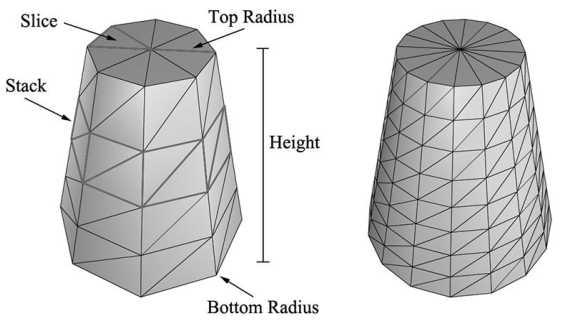
\includegraphics[width=\textwidth]{7-1}
    \centering
    \caption{在此图中,左侧的圆柱体有八个切片和四个堆叠,右侧的圆柱体有十六个切片和八个堆叠。 切片和堆栈控制三角形密度。 请注意,顶部和底部半径可以不同,以便我们可以创建锥形对象,而不仅仅是“纯”圆柱体。}
    \label{fig:7-1}
\end{figure}

%---- 7.4.1.1 ----
\subsubsection{圆柱体边缘几何(Cylinder Side Geometry)}
\begin{flushleft}
我们生成以原点为中心的圆柱体,平行于$y$轴。 从图\ref{fig:7-1}中,所有顶点都位于圆柱体的“环”上,其中有stackCount + 1个环,每个环都有 sliceCount 个(唯一)顶点。 连续环之间的半径差异为$\Delta r=(topRadius - bottomRadius)/ stackCount$。 如果我们从索引为0的底环开始,那么第i个环的半径是$r_{i} = bottomRadius + i\Delta r$,第i个环的高度是 $h_{i}=-\frac{h}{2}+i\Delta h$其中$\Delta h$是堆栈高度,h是圆柱高度。 因此,基本思想是迭代每个环,并生成位于该环上的顶点。 这给出了以下实现:\\
\end{flushleft}
\begin{lstlisting}
GeometryGenerator::MeshData 
GeometryGenerator::CreateCylinder(
    float bottomRadius, 
    float topRadius, 
    float height, 
    uint32 sliceCount, 
    uint32 stackCount)
{
    MeshData meshData;

    //
    // Build Stacks.
    // 

    float stackHeight = height / stackCount;

    // Amount to increment radius as we move up 
    // each stack level from bottom to top.
    float radiusStep = (topRadius - bottomRadius) / stackCount;

    uint32 ringCount = stackCount+1;

    // Compute vertices for each stack ring 
    // starting at the bottom and moving up.
    for(uint32 i = 0; i < ringCount; ++i)
    {
        float y = -0.5f*height + i*stackHeight;
        float r = bottomRadius + i*radiusStep;

        // vertices of ring
        float dTheta = 2.0f*XM_PI/sliceCount;
        for(uint32 j = 0; j <= sliceCount; ++j)
        {
            Vertex vertex;

            float c = cosf(j*dTheta);
            float s = sinf(j*dTheta);

            vertex.Position = XMFLOAT3(r*c, y, r*s);

            vertex.TexC.x = (float)j/sliceCount;
            vertex.TexC.y = 1.0f - (float)i/stackCount;

            // Cylinder can be parameterized as follows, where we introduce v
            // parameter that goes in the same direction as the v tex-coord
            // so that the bitangent goes in the same direction 
            // as the v tex-coord.
            //   Let r0 be the bottom radius and let r1 be the top radius.
            //   y(v) = h - hv for v in [0,1].
            //   r(v) = r1 + (r0-r1)v
            //
            //   x(t, v) = r(v)*cos(t)
            //   y(t, v) = h - hv
            //   z(t, v) = r(v)*sin(t)
            // 
            //  dx/dt = -r(v)*sin(t)
            //  dy/dt = 0
            //  dz/dt = +r(v)*cos(t)
            //
            //  dx/dv = (r0-r1)*cos(t)
            //  dy/dv = -h
            //  dz/dv = (r0-r1)*sin(t)

            // This is unit length.
            vertex.TangentU = XMFLOAT3(-s, 0.0f, c);

            float dr = bottomRadius-topRadius;
            XMFLOAT3 bitangent(dr*c, -height, dr*s);

            XMVECTOR T = XMLoadFloat3(&vertex.TangentU);
            XMVECTOR B = XMLoadFloat3(&bitangent);
            XMVECTOR N = XMVector3Normalize(XMVector3Cross(T, B));
            XMStoreFloat3(&vertex.Normal, N);

            meshData.Vertices.push_back(vertex);
        }
    }
......
\end{lstlisting}
\begin{flushleft}
NOTICE: 观察到每个环的第一个和最后一个顶点在位置上重复,但纹理坐标不重复。 我们必须这样做,以便我们可以正确地将纹理应用于圆柱体。\\
~\\
NOTICE: 实际上GeometryGenerator::CreateCylinder创建了额外的顶点数据,例如法线向量和纹理坐标,这些对未来的演示非常有用。 现在不要担心这些数量。\\
~\\
从图\ref{fig:7-2}可以看出,每个堆栈中的每个切片都有一个四边形(两个三角形)。 图\ref{fig:7-2}显示第$i$个堆栈和第$j$个切片的索引由下式给出:\\
\end{flushleft}
\begin{align*}
\Delta ABC = (i\cdot n+j, (i+1)\cdot n+j,(i+1)\cdot n+j+1)\\
\Delta ACD = (i\cdot n+j, (i+1)\cdot n+j+1,i\cdot n+j+1)
\end{align*}
\begin{flushleft}
其中n是每个环的顶点数。 所以关键的想法是遍历每个堆栈中的每个切片,并应用上面的公式。\\
\end{flushleft}
\begin{lstlisting}
    // Add one because we duplicate the first and last vertex per ring
    // since the texture coordinates are different.
    uint32 ringVertexCount = sliceCount+1;

    // Compute indices for each stack.
    for(uint32 i = 0; i < stackCount; ++i)
    {
        for(uint32 j = 0; j < sliceCount; ++j)
        {
            meshData.Indices32.push_back(i*ringVertexCount + j);
            meshData.Indices32.push_back((i+1)*ringVertexCount + j);
            meshData.Indices32.push_back((i+1)*ringVertexCount + j+1);

            meshData.Indices32.push_back(i*ringVertexCount + j);
            meshData.Indices32.push_back((i+1)*ringVertexCount + j+1);
            meshData.Indices32.push_back(i*ringVertexCount + j+1);
        }
    }

    BuildCylinderTopCap(bottomRadius, topRadius, height, sliceCount, stackCount, meshData);
    BuildCylinderBottomCap(bottomRadius, topRadius, height, sliceCount, stackCount, meshData);

    return meshData;
}
\end{lstlisting}
\begin{figure}[h]
    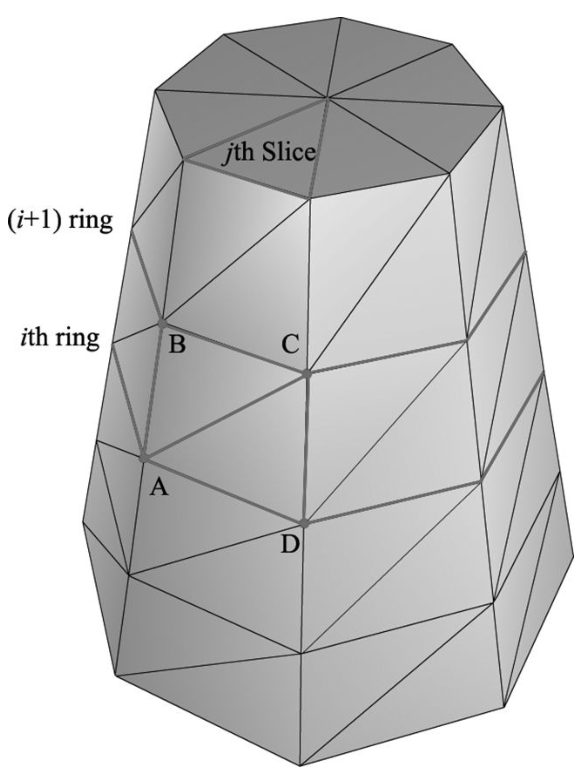
\includegraphics[width=\textwidth]{7-2}
    \centering
    \caption{包含在第$i$个和第$i + 1$个环中的顶点A,B,C,D和第$j$个切片。}
    \label{fig:7-2}
\end{figure}

%---- 7.4.1.2 ----
\subsubsection{顶面底面几何(Cap Geometry)}
\begin{flushleft}
生成顶面几何图形相当于生成顶部和底部环的切片三角形以近似圆形:\\
\end{flushleft}
\begin{lstlisting}
void GeometryGenerator::BuildCylinderTopCap(
    float bottomRadius, 
    float topRadius, 
    float height,
    uint32 sliceCount, 
    uint32 stackCount, 
    MeshData& meshData)
{
    uint32 baseIndex = (uint32)meshData.Vertices.size();

    float y = 0.5f*height;
    float dTheta = 2.0f*XM_PI/sliceCount;

    // Duplicate cap ring vertices because 
    // the texture coordinates and normals differ.
    for(uint32 i = 0; i <= sliceCount; ++i)
    {
        float x = topRadius*cosf(i*dTheta);
        float z = topRadius*sinf(i*dTheta);

        // Scale down by the height to try and 
        // make top cap texture coord area
        // proportional to base.
        float u = x/height + 0.5f;
        float v = z/height + 0.5f;

        meshData.Vertices.push_back(
            Vertex(x, y, z, 
                0.0f, 1.0f, 0.0f, 
                1.0f, 0.0f, 0.0f, 
                u, v));
    }

    // Cap center vertex.
    meshData.Vertices.push_back(
        Vertex(0.0f, y, 0.0f, 
            0.0f, 1.0f, 0.0f, 
            1.0f, 0.0f, 0.0f, 
            0.5f, 0.5f));

    // Index of center vertex.
    uint32 centerIndex = (uint32)meshData.Vertices.size()-1;

    for(uint32 i = 0; i < sliceCount; ++i)
    {
        meshData.Indices32.push_back(centerIndex);
        meshData.Indices32.push_back(baseIndex + i+1);
        meshData.Indices32.push_back(baseIndex + i);
    }
}
\end{lstlisting}
\begin{flushleft}
底面类似。\\
\end{flushleft}

%---- 7.4.2 ----
\subsection{创建球面网格(Generating a Sphere Mesh)}
\begin{flushleft}
我们通过指定半径,切片和堆栈计数来定义球体,如图\ref{fig:7-3}所示。 除了每个环的半径变化是基于三角函数的非线性方式之外,用于生成球体的算法非常类似于圆柱体的算法。 我们将留给读者研究 GeometryGenerator::CreateSphere 代码。 请注意,我们可以应用非均匀缩放世界变换将球体变换为椭圆体。
\end{flushleft}
\begin{figure}[h]
    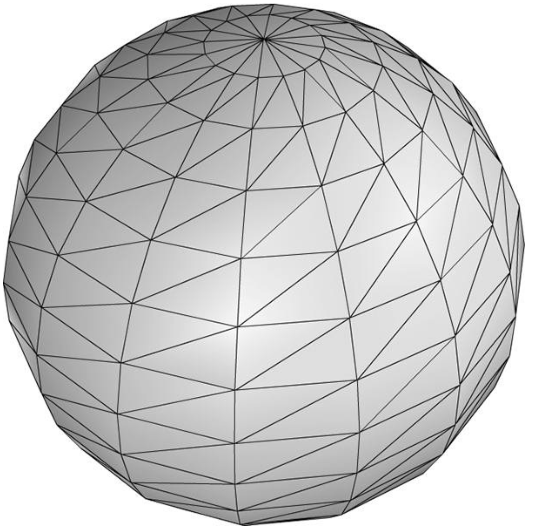
\includegraphics[width=\textwidth]{7-3}
    \centering
    \caption{切片和堆栈的思想也适用于球体来控制曲面细分的级别。}
    \label{fig:7-3}
\end{figure}

%---- 7.4.3 ----
\subsection{创建地圈网格(Generating a Geosphere Mesh)}
\begin{flushleft}
从图\ref{fig:7-3}可以看出,球体的三角形没有相等的面积。 在某些情况下这可能是不合需要的。 地圈使用具有几乎相等面积的三角形以及相等的边长来近似球体(参见图\ref{fig:7-4})。
\end{flushleft}

\begin{figure}[h]
    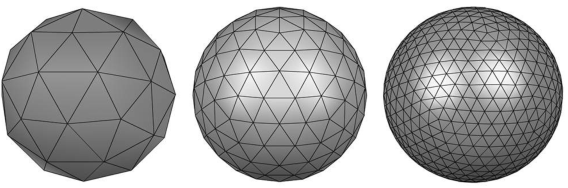
\includegraphics[width=\textwidth]{7-4}
    \centering
    \caption{通过重复细分和重投影到球体上来近似地圈。}
    \label{fig:7-4}
\end{figure}

\begin{flushleft}
为了生成地圈,我们从二十面体开始,细分三角形,然后将新顶点投影到具有给定半径的球体上。 我们可以重复此过程以改进曲面细分。\\
图\ref{fig:7-5}显示了如何将三角形细分为四个相等大小的三角形。 只需沿原始三角形的边缘取中点即可找到新的顶点。 然后,通过将顶点投影到单位球上然后标量乘以$r: v^{'}=r \frac{v}{||v||}$,可以将新顶点投影到半径为$r$的球体上
\end{flushleft}

\begin{figure}[h]
    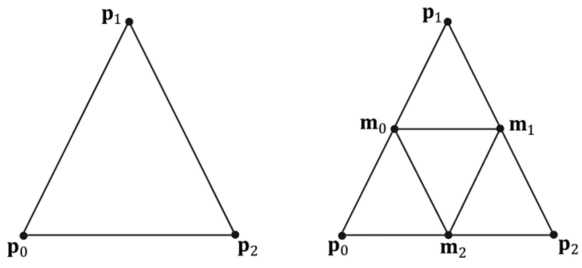
\includegraphics[width=\textwidth]{7-5}
    \centering
    \caption{将三角形细分为四个相等面积的三角形。}
    \label{fig:7-5}
\end{figure}

\begin{flushleft}
代码如下:\\
\end{flushleft}
\begin{lstlisting}
GeometryGenerator::MeshData 
GeometryGenerator::CreateGeosphere(
    float radius, 
    uint32 numSubdivisions)
{
    MeshData meshData;

    // Put a cap on the number of subdivisions.
    numSubdivisions = std::min<uint32>(numSubdivisions, 6u);

    // Approximate a sphere by tessellating an icosahedron.

    const float X = 0.525731f; 
    const float Z = 0.850651f;

    XMFLOAT3 pos[12] = 
    {
        XMFLOAT3(-X, 0.0f, Z),  XMFLOAT3(X, 0.0f, Z),  
        XMFLOAT3(-X, 0.0f, -Z), XMFLOAT3(X, 0.0f, -Z),    
        XMFLOAT3(0.0f, Z, X),   XMFLOAT3(0.0f, Z, -X), 
        XMFLOAT3(0.0f, -Z, X),  XMFLOAT3(0.0f, -Z, -X),    
        XMFLOAT3(Z, X, 0.0f),   XMFLOAT3(-Z, X, 0.0f), 
        XMFLOAT3(Z, -X, 0.0f),  XMFLOAT3(-Z, -X, 0.0f)
    };

    uint32 k[60] =
    {
        1,4,0,  4,9,0,  4,5,9,  8,5,4,  1,8,4,    
        1,10,8, 10,3,8, 8,3,5,  3,2,5,  3,7,2,    
        3,10,7, 10,6,7, 6,11,7, 6,0,11, 6,1,0, 
        10,1,6, 11,0,9, 2,11,9, 5,2,9,  11,2,7 
    };

    meshData.Vertices.resize(12);
    meshData.Indices32.assign(&k[0], &k[60]);

    for(uint32 i = 0; i < 12; ++i)
        meshData.Vertices[i].Position = pos[i];

    for(uint32 i = 0; i < numSubdivisions; ++i)
        Subdivide(meshData);

    // Project vertices onto sphere and scale.
    for(uint32 i = 0; i < meshData.Vertices.size(); ++i)
    {
        // Project onto unit sphere.
        XMVECTOR n = XMVector3Normalize(XMLoadFloat3(&meshData.Vertices[i].Position));

        // Project onto sphere.
        XMVECTOR p = radius*n;

        XMStoreFloat3(&meshData.Vertices[i].Position, p);
        XMStoreFloat3(&meshData.Vertices[i].Normal, n);

        // Derive texture coordinates from spherical coordinates.
        float theta = atan2f(meshData.Vertices[i].Position.z, 
                             meshData.Vertices[i].Position.x);

        // Put in [0, 2pi].
        if(theta < 0.0f)
            theta += XM_2PI;

        float phi = acosf(meshData.Vertices[i].Position.y / radius);

        meshData.Vertices[i].TexC.x = theta/XM_2PI;
        meshData.Vertices[i].TexC.y = phi/XM_PI;

        // Partial derivative of P with respect to theta
        meshData.Vertices[i].TangentU.x = -radius*sinf(phi)*sinf(theta);
        meshData.Vertices[i].TangentU.y = 0.0f;
        meshData.Vertices[i].TangentU.z = +radius*sinf(phi)*cosf(theta);

        XMVECTOR T = XMLoadFloat3(&meshData.Vertices[i].TangentU);
        XMStoreFloat3(&meshData.Vertices[i].TangentU, XMVector3Normalize(T));
    }

    return meshData;
}
\end{lstlisting}

%---- 7.5 ----
\section{Shapes Demo}
\begin{flushleft}
为了演示我们的球体和圆柱体生成代码,我们实现了如图\ref{fig:7-6}所示的 "Shapes" 演示。 此外,您还将获得在场景中定位和绘制多个对象的经验(即,创建多个世界变换矩阵)。 此外,我们将所有场景几何体放在一个大顶点和索引缓冲区中。 然后我们将使用 DrawIndexedInstanced 方法一次绘制一个对象(因为需要在对象之间更改世界矩阵); 因此,您将看到使用 DrawIndexedInstanced 的 StartIndexLocation 和 BaseVertexLocation 参数的示例。\\
\end{flushleft}

\begin{figure}[h]
    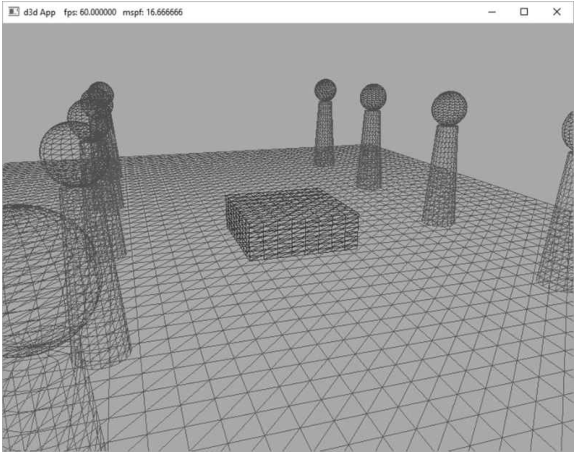
\includegraphics[width=\textwidth]{7-6}
    \centering
    \caption{"Shapes"演示的截图}
    \label{fig:7-6}
\end{figure}

%---- 7.5.1 ----
\subsection{顶点和顶点缓冲区(Vertex and Index Buffers)}
\begin{flushleft}
如图\ref{fig:7-6}所示,在本演示中,我们绘制了一个框,网格(grid),圆柱体和球体。 尽管我们在此演示中绘制了多个球体和圆柱体,但我们只需要一个球体和圆柱体几何体的副本。 我们只是多次重绘相同的球体和圆柱网格,但是使用不同的世界矩阵; 这是几何实例化的一个例子,它可以节省内存。\\
我们将所有网格顶点和索引打包到一个顶点和索引缓冲区中。 这是通过连接顶点和索引数组来完成的。 这意味着当我们绘制一个对象时,我们只绘制顶点和索引缓冲区的子集。 为了使用 ID3D12CommandList::DrawIndexedInstanced 仅绘制几何的子集,我们需要知道三个量(回想一下图\ref{fig:6-3}以及第6章中关于它的讨论)。 我们需要知道连接索引缓冲区中对象的起始索引,它的索引计数,我们需要知道基本顶点位置 - 对象相对于连接顶点缓冲区的第一个顶点的索引。 回想一下,基本顶点位置是在提取顶点之前添加到绘制调用中的索引的整数值,以便索引引用连接顶点缓冲区中的正确子集。 (另见第5章的练习2)\\

下面的代码显示了如何创建几何缓冲区,如何缓存必要的图纸数量以及如何绘制对象。
\end{flushleft}

\begin{lstlisting}
void ShapesApp::BuildShapeGeometry()
{
    GeometryGenerator geoGen;
    GeometryGenerator::MeshData box = 
        geoGen.CreateBox(1.5f, 0.5f, 1.5f, 3);
    GeometryGenerator::MeshData grid = 
        geoGen.CreateGrid(20.0f, 30.0f, 60, 40);
    GeometryGenerator::MeshData sphere = 
        geoGen.CreateSphere(0.5f, 20, 20);
    GeometryGenerator::MeshData cylinder = 
        geoGen.CreateCylinder(0.5f, 0.3f, 3.0f, 20, 20);

    //
    // We are concatenating all the geometry 
    // into one big vertex/index buffer.  So
    // define the regions in the buffer each submesh covers.
    //

    // Cache the vertex offsets to each object 
    // in the concatenated vertex buffer.
    UINT boxVertexOffset = 0;
    UINT gridVertexOffset = (UINT)box.Vertices.size();
    UINT sphereVertexOffset = gridVertexOffset + 
                           (UINT)grid.Vertices.size();
    UINT cylinderVertexOffset = sphereVertexOffset + 
                           (UINT)sphere.Vertices.size();

    // Cache the starting index for each object in the concatenated index buffer.
    UINT boxIndexOffset = 0;
    UINT gridIndexOffset = (UINT)box.Indices32.size();
    UINT sphereIndexOffset = gridIndexOffset + 
                           (UINT)grid.Indices32.size();
    UINT cylinderIndexOffset = sphereIndexOffset + 
                           (UINT)sphere.Indices32.size();

    // Define the SubmeshGeometry that cover different 
    // regions of the vertex/index buffers.

    SubmeshGeometry boxSubmesh;
    boxSubmesh.IndexCount = (UINT)box.Indices32.size();
    boxSubmesh.StartIndexLocation = boxIndexOffset;
    boxSubmesh.BaseVertexLocation = boxVertexOffset;

    SubmeshGeometry gridSubmesh;
    gridSubmesh.IndexCount = (UINT)grid.Indices32.size();
    gridSubmesh.StartIndexLocation = gridIndexOffset;
    gridSubmesh.BaseVertexLocation = gridVertexOffset;

    SubmeshGeometry sphereSubmesh;
    sphereSubmesh.IndexCount = (UINT)sphere.Indices32.size();
    sphereSubmesh.StartIndexLocation = sphereIndexOffset;
    sphereSubmesh.BaseVertexLocation = sphereVertexOffset;

    SubmeshGeometry cylinderSubmesh;
    cylinderSubmesh.IndexCount = (UINT)cylinder.Indices32.size();
    cylinderSubmesh.StartIndexLocation = cylinderIndexOffset;
    cylinderSubmesh.BaseVertexLocation = cylinderVertexOffset;

    //
    // Extract the vertex elements we are 
    // interested in and pack the
    // vertices of all the meshes into 
    // one vertex buffer.
    //

    auto totalVertexCount =
        box.Vertices.size() +
        grid.Vertices.size() +
        sphere.Vertices.size() +
        cylinder.Vertices.size();

    std::vector<Vertex> vertices(totalVertexCount);

    UINT k = 0;
    for(size_t i = 0; i < box.Vertices.size(); ++i, ++k)
    {
        vertices[k].Pos = box.Vertices[i].Position;
        vertices[k].Color = XMFLOAT4(DirectX::Colors::DarkGreen);
    }

    for(size_t i = 0; i < grid.Vertices.size(); ++i, ++k)
    {
        vertices[k].Pos = grid.Vertices[i].Position;
        vertices[k].Color = XMFLOAT4(DirectX::Colors::ForestGreen);
    }

    for(size_t i = 0; i < sphere.Vertices.size(); ++i, ++k)
    {
        vertices[k].Pos = sphere.Vertices[i].Position;
        vertices[k].Color = XMFLOAT4(DirectX::Colors::Crimson);
    }

    for(size_t i = 0; i < cylinder.Vertices.size(); ++i, ++k)
    {
        vertices[k].Pos = cylinder.Vertices[i].Position;
        vertices[k].Color = XMFLOAT4(DirectX::Colors::SteelBlue);
    }

    std::vector<std::uint16_t> indices;
    indices.insert(indices.end(), 
                   std::begin(box.GetIndices16()), 
                   std::end(box.GetIndices16()));
    indices.insert(indices.end(), 
                   std::begin(grid.GetIndices16()), 
                   std::end(grid.GetIndices16()));
    indices.insert(indices.end(), 
                   std::begin(sphere.GetIndices16()), 
                   std::end(sphere.GetIndices16()));
    indices.insert(indices.end(), 
                   std::begin(cylinder.GetIndices16()), 
                   std::end(cylinder.GetIndices16()));

    const UINT vbByteSize = (UINT)vertices.size() * 
                            sizeof(Vertex);
    const UINT ibByteSize = (UINT)indices.size() * 
                            sizeof(std::uint16_t);

    auto geo = std::make_unique<MeshGeometry>();
    geo->Name = "shapeGeo";

    ThrowIfFailed(D3DCreateBlob(vbByteSize, &geo->VertexBufferCPU));
    CopyMemory(geo->VertexBufferCPU->GetBufferPointer(), 
                    vertices.data(), 
                    vbByteSize);

    ThrowIfFailed(D3DCreateBlob(ibByteSize, &geo->IndexBufferCPU));
    CopyMemory(geo->IndexBufferCPU->GetBufferPointer(), 
                    indices.data(), 
                    ibByteSize);

    geo->VertexBufferGPU = d3dUtil::CreateDefaultBuffer(md3dDevice.Get(),
        mCommandList.Get(), vertices.data(), 
        vbByteSize, geo->VertexBufferUploader);

    geo->IndexBufferGPU = d3dUtil::CreateDefaultBuffer(md3dDevice.Get(),
        mCommandList.Get(), indices.data(), 
        ibByteSize, geo->IndexBufferUploader);

    geo->VertexByteStride = sizeof(Vertex);
    geo->VertexBufferByteSize = vbByteSize;
    geo->IndexFormat = DXGI_FORMAT_R16_UINT;
    geo->IndexBufferByteSize = ibByteSize;

    geo->DrawArgs["box"] = boxSubmesh;
    geo->DrawArgs["grid"] = gridSubmesh;
    geo->DrawArgs["sphere"] = sphereSubmesh;
    geo->DrawArgs["cylinder"] = cylinderSubmesh;

    mGeometries[geo->Name] = std::move(geo);
}
\end{lstlisting}

\begin{flushleft}
在上面方法的最后一行中使用的 mGeometries 变量定义如下:\\
\end{flushleft}

\begin{lstlisting}
std::unordered_map<std::string, 
            std::unique_ptr<MeshGeometry>> mGeometries;
\end{lstlisting}

\begin{flushleft}
这是我们在本书其余部分使用的常见模式。 为每个几何体,PSO,纹理,着色器等创建新的变量名称很麻烦,因此我们使用无序地图进行常量时间查找并按名称引用我们的对象。 以下是一些例子:\\
\end{flushleft}

\begin{lstlisting}
std::unordered_map<std::string,
    std::unique_ptr<MeshGeometry>> mGeometries;
std::unordered_map<std::string, ComPtr<ID3DBlob>>
    mShaders;
std::unordered_map<std::string,
    ComPtr<ID3D12PipelineState>> mPSOs;
\end{lstlisting}

%---- 7.5.2 ----
\subsection{渲染项(Render Items)}
\begin{flushleft}
我们现在定义场景渲染项。 观察所有渲染项如何共享相同的 MeshGeometry,并使用 DrawArgs 获取 DrawIndexedInstanced 参数以绘制顶点/索引缓冲区的子区域。\\
\end{flushleft}

\begin{lstlisting}
// ShapesApp member variable.
std::vector<std::unique_ptr<RenderItem>> mAllRitems;
std::vector<RenderItem*> mOpaqueRitems;

void ShapesApp::BuildRenderItems()
{
    auto boxRitem = std::make_unique<RenderItem>();
    XMStoreFloat4x4(&boxRitem->World, 
         XMMatrixScaling(2.0f, 2.0f, 2.0f)*
         XMMatrixTranslation(0.0f, 0.5f, 0.0f));

    boxRitem->ObjCBIndex = 0;
    boxRitem->Geo = mGeometries["shapeGeo"].get();
    boxRitem->PrimitiveType = D3D_PRIMITIVE_TOPOLOGY_TRIANGLELIST;
    boxRitem->IndexCount = boxRitem->Geo->
        DrawArgs["box"].IndexCount;
    boxRitem->StartIndexLocation = boxRitem->Geo->
        DrawArgs["box"].StartIndexLocation;
    boxRitem->BaseVertexLocation = boxRitem->Geo->
        DrawArgs["box"].BaseVertexLocation;
    mAllRitems.push_back(std::move(boxRitem));

    auto gridRitem = std::make_unique<RenderItem>();
    gridRitem->World = MathHelper::Identity4x4();
    gridRitem->ObjCBIndex = 1;
    gridRitem->Geo = mGeometries["shapeGeo"].get();
    gridRitem->PrimitiveType = D3D_PRIMITIVE_TOPOLOGY_TRIANGLELIST;
    gridRitem->IndexCount = gridRitem->Geo->
        DrawArgs["grid"].IndexCount;
    gridRitem->StartIndexLocation = gridRitem->Geo->
        DrawArgs["grid"].StartIndexLocation;
    gridRitem->BaseVertexLocation = gridRitem->Geo->
        DrawArgs["grid"].BaseVertexLocation;
    mAllRitems.push_back(std::move(gridRitem));

    UINT objCBIndex = 2;
    for(int i = 0; i < 5; ++i)
    {
        auto leftCylRitem = std::make_unique<RenderItem>();
        auto rightCylRitem = std::make_unique<RenderItem>();
        auto leftSphereRitem = std::make_unique<RenderItem>();
        auto rightSphereRitem = std::make_unique<RenderItem>();

        XMMATRIX leftCylWorld = XMMatrixTranslation(
            -5.0f, 1.5f, -10.0f + i*5.0f);
        XMMATRIX rightCylWorld = XMMatrixTranslation(
            +5.0f, 1.5f, -10.0f + i*5.0f);

        XMMATRIX leftSphereWorld = XMMatrixTranslation(
            -5.0f, 3.5f, -10.0f + i*5.0f);
        XMMATRIX rightSphereWorld = XMMatrixTranslation(
            +5.0f, 3.5f, -10.0f + i*5.0f);

        XMStoreFloat4x4(&leftCylRitem->World, 
            rightCylWorld);
        leftCylRitem->ObjCBIndex = objCBIndex++;
        leftCylRitem->Geo = mGeometries["shapeGeo"].get();
        leftCylRitem->PrimitiveType = 
            D3D_PRIMITIVE_TOPOLOGY_TRIANGLELIST;
        leftCylRitem->IndexCount = leftCylRitem->Geo->
            DrawArgs["cylinder"].IndexCount;
        leftCylRitem->StartIndexLocation = leftCylRitem->Geo->
            DrawArgs["cylinder"].StartIndexLocation;
        leftCylRitem->BaseVertexLocation = leftCylRitem->Geo->
            DrawArgs["cylinder"].BaseVertexLocation;

        XMStoreFloat4x4(&rightCylRitem->World, leftCylWorld);
        rightCylRitem->ObjCBIndex = objCBIndex++;
        rightCylRitem->Geo = mGeometries["shapeGeo"].get();
        rightCylRitem->PrimitiveType = 
            D3D_PRIMITIVE_TOPOLOGY_TRIANGLELIST;
        rightCylRitem->IndexCount = rightCylRitem->Geo->
            DrawArgs["cylinder"].IndexCount;
        rightCylRitem->StartIndexLocation = rightCylRitem->Geo->
            DrawArgs["cylinder"].StartIndexLocation;
        rightCylRitem->BaseVertexLocation = rightCylRitem->Geo->
            DrawArgs["cylinder"].BaseVertexLocation;

        XMStoreFloat4x4(&leftSphereRitem->World, leftSphereWorld);
        leftSphereRitem->ObjCBIndex = objCBIndex++;
        leftSphereRitem->Geo = mGeometries["shapeGeo"].get();
        leftSphereRitem->PrimitiveType = 
            D3D_PRIMITIVE_TOPOLOGY_TRIANGLELIST;
        leftSphereRitem->IndexCount = leftSphereRitem->Geo->
            DrawArgs["sphere"].IndexCount;
        leftSphereRitem->StartIndexLocation = leftSphereRitem->Geo->
            DrawArgs["sphere"].StartIndexLocation;
        leftSphereRitem->BaseVertexLocation = leftSphereRitem->Geo->
            DrawArgs["sphere"].BaseVertexLocation;

        XMStoreFloat4x4(&rightSphereRitem->World, rightSphereWorld);
        rightSphereRitem->ObjCBIndex = objCBIndex++;
        rightSphereRitem->Geo = mGeometries["shapeGeo"].get();
        rightSphereRitem->PrimitiveType = 
            D3D_PRIMITIVE_TOPOLOGY_TRIANGLELIST;
        rightSphereRitem->IndexCount = rightSphereRitem->Geo->
            DrawArgs["sphere"].IndexCount;
        rightSphereRitem->StartIndexLocation = rightSphereRitem->Geo->
            DrawArgs["sphere"].StartIndexLocation;
        rightSphereRitem->BaseVertexLocation = rightSphereRitem->Geo->
            DrawArgs["sphere"].BaseVertexLocation;

        mAllRitems.push_back(std::move(leftCylRitem));
        mAllRitems.push_back(std::move(rightCylRitem));
        mAllRitems.push_back(std::move(leftSphereRitem));
        mAllRitems.push_back(std::move(rightSphereRitem));
    }

    // All the render items are opaque.
    for(auto& e : mAllRitems)
        mOpaqueRitems.push_back(e.get());
}
\end{lstlisting}

%---- 7.5.3 ----
\subsection{帧资源和常量缓冲视图(Frame Resources and Constant Buffer Views)}
\begin{flushleft}
回想一下,我们有一个 FrameResources 的向量,每个 FrameResource 都有一个上传缓冲区,用于存储场景中每个渲染项的传递常量和常量缓冲区。
\end{flushleft}

\begin{lstlisting}
std::unique_ptr<UploadBuffer<PassConstants>> PassCB = nullptr;
std::unique_ptr<UploadBuffer<ObjectConstants>> ObjectCB = nullptr;
\end{lstlisting}

\begin{flushleft}
如果我们有3个帧资源和 $n$ 个渲染项,那么我们有 $3n$ 个对象\footnote{原文是:"then we have three 3n object constant
buffers",是错误的}常量缓冲区和3个传递常量缓冲区。 因此,我们需要$3(n+1)$个常量缓冲区视图(CBV)。 所以,我们需要修改我们的CBV堆以包含其他描述符:\\
\end{flushleft}

\begin{lstlisting}
void ShapesApp::BuildDescriptorHeaps()
{
    UINT objCount = (UINT)mOpaqueRitems.size();

    // Need a CBV descriptor for each object for each frame resource,
    // +1 for the perPass CBV for each frame resource.
    UINT numDescriptors = (objCount+1) * 3;

    // Save an offset to the start of the pass CBVs.  
    // These are the last 3 descriptors.
    mPassCbvOffset = objCount * gNumFrameResources;

    D3D12_DESCRIPTOR_HEAP_DESC cbvHeapDesc;
    cbvHeapDesc.NumDescriptors = numDescriptors;
    cbvHeapDesc.Type = D3D12_DESCRIPTOR_HEAP_TYPE_CBV_SRV_UAV;
    cbvHeapDesc.Flags = D3D12_DESCRIPTOR_HEAP_FLAG_SHADER_VISIBLE;
    cbvHeapDesc.NodeMask = 0;
    ThrowIfFailed(md3dDevice->CreateDescriptorHeap(&cbvHeapDesc,
        IID_PPV_ARGS(&mCbvHeap)));
}
\end{lstlisting}

\begin{flushleft}
现在,我们可以使用以下代码填充CBV堆,其中描述符$0$到$n-1$包含第$0$帧资源的对象CBV,描述符$n$到$2n-1$包含第$1$帧资源的对象CBV,描述符$2n$到$3n-1$ 包含第二帧资源的对象CBV,描述符$3n$,$3n + 1$和$3n + 2$分别包含第$0$帧,第$1$帧和第$2$帧资源的传递CBV:\\
\end{flushleft}

\begin{lstlisting}
void ShapesApp::BuildConstantBufferViews()
{
    UINT objCBByteSize = d3dUtil::CalcConstantBufferByteSize(
            sizeof(ObjectConstants));

    UINT objCount = (UINT)mOpaqueRitems.size();

    // Need a CBV descriptor for each object for each frame resource.
    for(int frameIndex = 0; 
        frameIndex < gNumFrameResources; 
        ++frameIndex)
    {
        auto objectCB = mFrameResources[frameIndex]->
            ObjectCB->Resource();
        for(UINT i = 0; i < objCount; ++i)
        {
            D3D12_GPU_VIRTUAL_ADDRESS cbAddress = 
                objectCB->GetGPUVirtualAddress();

            // Offset to the ith object constant buffer in the buffer.
            cbAddress += i*objCBByteSize;

            // Offset to the object cbv in the descriptor heap.
            int heapIndex = frameIndex*objCount + i;
            auto handle = CD3DX12_CPU_DESCRIPTOR_HANDLE(mCbvHeap->
                GetCPUDescriptorHandleForHeapStart());
            handle.Offset(heapIndex, mCbvSrvUavDescriptorSize);

            D3D12_CONSTANT_BUFFER_VIEW_DESC cbvDesc;
            cbvDesc.BufferLocation = cbAddress;
            cbvDesc.SizeInBytes = objCBByteSize;

            md3dDevice->CreateConstantBufferView(&cbvDesc, handle);
        }
    }

    UINT passCBByteSize = d3dUtil::CalcConstantBufferByteSize(
        sizeof(PassConstants));

    // Last three descriptors are the pass CBVs for each frame resource.
    for(int frameIndex = 0; frameIndex < gNumFrameResources; ++frameIndex)
    {
        auto passCB = mFrameResources[frameIndex]->PassCB->Resource();
        D3D12_GPU_VIRTUAL_ADDRESS cbAddress = passCB->GetGPUVirtualAddress();

        // Offset to the pass cbv in the descriptor heap.
        int heapIndex = mPassCbvOffset + frameIndex;
        auto handle = CD3DX12_CPU_DESCRIPTOR_HANDLE(mCbvHeap->
            GetCPUDescriptorHandleForHeapStart());
        handle.Offset(heapIndex, mCbvSrvUavDescriptorSize);

        D3D12_CONSTANT_BUFFER_VIEW_DESC cbvDesc;
        cbvDesc.BufferLocation = cbAddress;
        cbvDesc.SizeInBytes = passCBByteSize;
        
        md3dDevice->CreateConstantBufferView(&cbvDesc, handle);
    }
}
\end{lstlisting}

\begin{flushleft}
回想一下,我们可以使用 ID3D12DescriptorHeap::GetCPUDescriptorHandleForHeapStart 方法获取堆中第一个描述符的句柄。 但是,现在我们的堆有多个描述符,这个方法已不再适用。 我们需要能够偏移到堆中的其他描述符。 为此,我们需要知道要在堆中递增的大小以获取到下一个描述符。 这是特定于硬件的,因此我们必须从设备查询此信息,这取决于堆类型。 回想一下,我们的 D3DApp 类缓存了这些信息:\\
\end{flushleft}

\begin{lstlisting}
mRtvDescriptorSize = md3dDevice->
    GetDescriptorHandleIncrementSize(
    D3D12_DESCRIPTOR_HEAP_TYPE_RTV);
mDsvDescriptorSize = md3dDevice->
    GetDescriptorHandleIncrementSize(
    D3D12_DESCRIPTOR_HEAP_TYPE_DSV);
mCbvSrvUavDescriptorSize = md3dDevice->
    GetDescriptorHandleIncrementSize(
    D3D12_DESCRIPTOR_HEAP_TYPE_CBV_SRV_UAV);
\end{lstlisting}

\begin{flushleft}
一旦我们知道描述符增量大小,我们就可以使用两个 CD3DX12\_CPU\_DESCRIPTOR\_HANDLE::Offset 方法之一来通过 n 个描述符来偏移句柄:\\
\end{flushleft}

\begin{lstlisting}
// Specify the number of descriptors to offset times 
// the descriptor Offset by n descriptors:
CD3DX12_CPU_DESCRIPTOR_HANDLE handle = mCbvHeap->
    GetCPUDescriptorHandleForHeapStart();
handle.Offset(n * mCbvSrvDescriptorSize);

// Or equivalently, specify the number of 
// descriptors to offset, followed by 
// the descriptor increment size:
CD3DX12_CPU_DESCRIPTOR_HANDLE handle = mCbvHeap->
    GetCPUDescriptorHandleForHeapStart();
handle.Offset(n, mCbvSrvDescriptorSize);
\end{lstlisting}

\begin{flushleft}
NOTICE: CD3DX12\_GPU\_DESCRIPTOR\_HANDLE 有相同的 Offset 方法。
\end{flushleft}


%---- 7.5.4 ----
\subsection{绘制场景(Draw the Scene)}
\begin{flushleft}
最后我们可以绘制渲染项。 也许唯一棘手的部分是通过程序偏移到堆中(我们想要绘制的对象的)正确CBV。 注意渲染项如何将索引存储到与渲染项关联的常量缓冲区的。\\
\end{flushleft}

\begin{lstlisting}
void ShapesApp::DrawRenderItems(
    ID3D12GraphicsCommandList* cmdList, 
    const std::vector<RenderItem*>& ritems)
{
    UINT objCBByteSize = d3dUtil::CalcConstantBufferByteSize(
        sizeof(ObjectConstants));
 
    auto objectCB = mCurrFrameResource->ObjectCB->Resource();

    // For each render item...
    for(size_t i = 0; i < ritems.size(); ++i)
    {
        auto ri = ritems[i];

        cmdList->IASetVertexBuffers(0, 1, 
            &ri->Geo->VertexBufferView());
        cmdList->IASetIndexBuffer(
            &ri->Geo->IndexBufferView());
        cmdList->IASetPrimitiveTopology(
            ri->PrimitiveType);

        // Offset to the CBV in the descriptor heap for 
        // this object and for this frame resource.
        UINT cbvIndex = mCurrFrameResourceIndex*
            (UINT)mOpaqueRitems.size() + ri->ObjCBIndex;
        auto cbvHandle = CD3DX12_GPU_DESCRIPTOR_HANDLE(mCbvHeap->
            GetGPUDescriptorHandleForHeapStart());
        cbvHandle.Offset(cbvIndex, mCbvSrvUavDescriptorSize);

        cmdList->SetGraphicsRootDescriptorTable(0, cbvHandle);

        cmdList->DrawIndexedInstanced(ri->IndexCount, 1, 
            ri->StartIndexLocation, ri->BaseVertexLocation, 0);
    }
}
\end{lstlisting}

\begin{flushleft}
DrawRenderItems 方法由 Draw 调用:\\
\end{flushleft}

\begin{lstlisting}
void ShapesApp::Draw(const GameTimer& gt)
{
    auto cmdListAlloc = mCurrFrameResource->CmdListAlloc;

    // Reuse the memory associated with command recording.
    // We can only reset when the associated command 
    // lists have finished execution on the GPU.
    ThrowIfFailed(cmdListAlloc->Reset());

    // A command list can be reset after it has 
    // been added to the command queue via ExecuteCommandList.
    // Reusing the command list reuses memory.
    if(mIsWireframe)
    {
        ThrowIfFailed(mCommandList->Reset(
            cmdListAlloc.Get(), 
            mPSOs["opaque_wireframe"].Get()));
    }
    else
    {
        ThrowIfFailed(mCommandList->Reset(
            cmdListAlloc.Get(), 
            mPSOs["opaque"].Get()));
    }

    mCommandList->RSSetViewports(1, &mScreenViewport);
    mCommandList->RSSetScissorRects(1, &mScissorRect);

    // Indicate a state transition on the resource usage.
    mCommandList->ResourceBarrier(1, 
        &CD3DX12_RESOURCE_BARRIER::Transition(
            CurrentBackBuffer(),
            D3D12_RESOURCE_STATE_PRESENT, 
            D3D12_RESOURCE_STATE_RENDER_TARGET));

    // Clear the back buffer and depth buffer.
    mCommandList->ClearRenderTargetView(CurrentBackBufferView(), 
        Colors::LightSteelBlue, 0, nullptr);
    mCommandList->ClearDepthStencilView(DepthStencilView(), 
        D3D12_CLEAR_FLAG_DEPTH | D3D12_CLEAR_FLAG_STENCIL, 
        1.0f, 0, 0, nullptr);

    // Specify the buffers we are going to render to.
    mCommandList->OMSetRenderTargets(1, &CurrentBackBufferView(), 
        true, &DepthStencilView());

    ID3D12DescriptorHeap* descriptorHeaps[] = { mCbvHeap.Get() };
    mCommandList->SetDescriptorHeaps(
        _countof(descriptorHeaps), 
        descriptorHeaps);

    mCommandList->SetGraphicsRootSignature(mRootSignature.Get());

    int passCbvIndex = mPassCbvOffset + mCurrFrameResourceIndex;
    auto passCbvHandle = CD3DX12_GPU_DESCRIPTOR_HANDLE(
        mCbvHeap->GetGPUDescriptorHandleForHeapStart());
    passCbvHandle.Offset(passCbvIndex, mCbvSrvUavDescriptorSize);
    mCommandList->SetGraphicsRootDescriptorTable(1, passCbvHandle);

    DrawRenderItems(mCommandList.Get(), mOpaqueRitems);

    // Indicate a state transition on the resource usage.
    mCommandList->ResourceBarrier(1, 
        &CD3DX12_RESOURCE_BARRIER::Transition(
            CurrentBackBuffer(),
            D3D12_RESOURCE_STATE_RENDER_TARGET, 
            D3D12_RESOURCE_STATE_PRESENT));

    // Done recording commands.
    ThrowIfFailed(mCommandList->Close());

    // Add the command list to the queue for execution.
    ID3D12CommandList* cmdsLists[] = { mCommandList.Get() };
    mCommandQueue->ExecuteCommandLists(_countof(cmdsLists), cmdsLists);

    // Swap the back and front buffers
    ThrowIfFailed(mSwapChain->Present(0, 0));
    mCurrBackBuffer = (mCurrBackBuffer + 1) % SwapChainBufferCount;

    // Advance the fence value to mark commands 
    // up to this fence point.
    mCurrFrameResource->Fence = ++mCurrentFence;
    
    // Add an instruction to the command queue 
    // to set a new fence point. 
    // Because we are on the GPU timeline, 
    // the new fence point won't be 
    // set until the GPU finishes processing all
    // the commands prior to this Signal().
    mCommandQueue->Signal(mFence.Get(), mCurrentFence);
}
\end{lstlisting}

%---- 7.6 ----
\section{更多关于根签名(More on Root Signatures)}
\begin{flushleft}
我们在前一章的第6.6.5节中介绍了根签名。 根签名定义在发出绘制调用之前需要将哪些资源绑定到管道以及这些资源如何映射到着色器输入寄存器。 需要绑定哪些资源取决于当前着色器程序所期望的资源。 创建PSO时,将验证根签名和着色器程序组合。
\end{flushleft}

%---- 7.6.1 ----
\subsection{根参数(Root Parameters)}
\begin{flushleft}
回想一下,根签名是由一组根参数定义的。 到目前为止,我们只创建了一个存储描述符表的根参数。 但是,root参数实际上可以是以下三种类型之一:\\
\end{flushleft}

\begin{itemize}
  \item 描述符表(Descriptor Table): 期望描述符表引用堆中的连续范围,该范围标识要绑定的资源。
  \item 根描述符(Root Descriptor | Inline Descriptor): 期望直接设置描述符以识别要绑定的资源; 描述符不需要在堆中。 只有 CBV 到常量缓冲区,SRV/UAV 到缓冲区可以绑定为根描述符。 特别是,这意味着 SRV 到纹理不能绑定为根描述符。
  \item 根常量(Root constant): 期望直接绑定的32位常量值列表。
\end{itemize}

\begin{flushleft}
出于性能考虑,可以将64个DWORD限制在根签名中。 这三种根参数具有以下内存消耗:\\
\end{flushleft}

\begin{itemize}
  \item 描述符表(Descriptor Table): 1 DWORD
  \item 根描述符(Root Descriptor): 2 DWORDs
  \item 根常量(Root constant): 每 32-bit 常量 1 DWORD
\end{itemize}

\begin{flushleft}
我们可以创建一个任意的根签名,只要我们不超过64个DWORD限制。 根常量非常方便,但它们的成本很快就会增加。 例如,如果我们需要的唯一常量数据是世界视图投影矩阵,我们可以使用16个根常量来存储它,这将使我们不需要涉及常量缓冲区和CBV堆。 但是,这会占我们根签名预算的四分之一。 使用根描述符只能是两个DWORD,描述符表只有一个DWORD。 随着我们的应用程序变得越来越复杂,我们的常量缓冲区数据将变得越来越大,并且我们不太可能只使用根常量。 在实际应用程序中,您可能会使用所有三种类型的根参数的组合。\\
在代码中,通过填写 CD3DX12\_ROOT\_PARAMETER 结构来描述根参数。 正如我们在 CD3DX 代码中看到的那样,CD3DX12\_ROOT\_PARAMETER 扩展了 D3D12\_ROOT\_PARAMETER 并添加了一些辅助初始化函数。\\
\end{flushleft}

\begin{lstlisting}
typedef struct D3D12_ROOT_PARAMETER
{
    D3D12_ROOT_PARAMETER_TYPE ParameterType;
    union
    {
        D3D12_ROOT_DESCRIPTOR_TABLE DescriptorTable;
        D3D12_ROOT_CONSTANTS Constants;
        D3D12_ROOT_DESCRIPTOR Descriptor;
    };
    D3D12_SHADER_VISIBILITY ShaderVisibility;
} D3D12_ROOT_PARAMETER;
\end{lstlisting}

\begin{itemize}
  \item 1.ParameterType: 以下枚举类型的成员,指示根参数类型(描述符表,根常量,CBV根描述符,SRV根描述符,UAV根描述符)。
  \begin{lstlisting}
    enum D3D12_ROOT_PARAMETER_TYPE
    {
        D3D12_ROOT_PARAMETER_TYPE_DESCRIPTOR_TABLE = 0,
        D3D12_ROOT_PARAMETER_TYPE_32BIT_CONSTANTS = 1,
        D3D12_ROOT_PARAMETER_TYPE_CBV = 2,
        D3D12_ROOT_PARAMETER_TYPE_SRV = 3 ,
        D3D12_ROOT_PARAMETER_TYPE_UAV = 4
    } D3D12_ROOT_PARAMETER_TYPE;
  \end{lstlisting}
  \item 2.DescriptorTable/Constants/Descriptor: 描述根参数的结构。您填写的联合成员取决于根参数类型。 7.6.2节,7.6.3节和7.6.4节讨论了这些结构。
  \item 3.ShaderVisibility: 以下枚举的成员,指定哪个着色器程序可以看到此根参数。 通常在本书中我们指定 D3D12\_SHADER\_VISIBILITY\_ALL。 但是,如果我们知道资源仅用于像素着色器,那么我们可以指定 D3D12\_SHADER\_VISIBILITY\_PIXEL。 限制根参数的可见性可能会促使一些优化。\\
  \begin{lstlisting}
    enum D3D12_SHADER_VISIBILITY
    {
        D3D12_SHADER_VISIBILITY_ALL = 0,
        D3D12_SHADER_VISIBILITY_VERTEX = 1,
        D3D12_SHADER_VISIBILITY_HULL = 2,
        D3D12_SHADER_VISIBILITY_DOMAIN = 3,
        D3D12_SHADER_VISIBILITY_GEOMETRY = 4,
        D3D12_SHADER_VISIBILITY_PIXEL = 5
    } D3D12_SHADER_VISIBILITY;
  \end{lstlisting}
\end{itemize}

%---- 7.6.2 ----
\subsection{描述符表(Descriptor Tables)}
\begin{flushleft}
通过填写 D3D12\_ROOT\_PARAMETER 的 DescriptorTable 成员来进一步定义描述符表根参数。\\
\end{flushleft}

\begin{lstlisting}
typedef struct D3D12_ROOT_DESCRIPTOR_TABLE
{
    UINT NumDescriptorRanges;
    const D3D12_DESCRIPTOR_RANGE *pDescriptorRanges;
} D3D12_ROOT_DESCRIPTOR_TABLE;
\end{lstlisting}

\begin{flushleft}
这只是指定 D3D12\_DESCRIPTOR\_RANGE 的数组和数组中的范围数。\\
D3D12\_DESCRIPTOR\_RANGE 结构定义如下:\\
\end{flushleft}

\begin{lstlisting}
typedef struct D3D12_DESCRIPTOR_RANGE
{
    D3D12_DESCRIPTOR_RANGE_TYPE RangeType;
    UINT NumDescriptors;
    UINT BaseShaderRegister;
    UINT RegisterSpace;
    UINT OffsetInDescriptorsFromTableStart;
} D3D12_DESCRIPTOR_RANGE;
\end{lstlisting}

\begin{itemize}
  \item 1.RangeType: 以下枚举类型的成员,指示此范围中的描述符类型:\\
  \begin{lstlisting}
    enum D3D12_DESCRIPTOR_RANGE_TYPE
    {
    D3D12_DESCRIPTOR_RANGE_TYPE_SRV = 0,
    D3D12_DESCRIPTOR_RANGE_TYPE_UAV = 1,
    D3D12_DESCRIPTOR_RANGE_TYPE_CBV = 2 ,
    D3D12_DESCRIPTOR_RANGE_TYPE_SAMPLER = 3
    } D3D12_DESCRIPTOR_RANGE_TYPE;
  \end{lstlisting}
  NOTICE: 采样器描述符在纹理章节中讨论。
  \item 2.NumDescriptors: 范围中的描述符个数
  \item 3.BaseShaderRegister: 基本着色器寄存器参数绑定到。 例如,如果将 NumDescriptors 设置为3,将 BaseShaderRegister 设置为 1,范围类型为 CBV(对于常量缓冲区),那么您将绑定到 HLSL 寄存器\\
  \begin{lstlisting}
    cbuffer cbA : register(b1) {…};
    cbuffer cbB : register(b2) {…};
    cbuffer cbC : register(b3) {…};
  \end{lstlisting}
  \item 4.RegisterSpace: 此属性为您提供另一个指定着色器寄存器的维度。 例如,以下两个寄存器似乎与寄存器槽t0重叠,但它们是不同的寄存器,因为它们位于不同的空间中:\\
  \begin{lstlisting}
    Texture2D gDiffuseMap :register(t0,space0);
    Texture2D gNormalMap : register(t0, space1);
  \end{lstlisting}
  \item 5.OffsetInDescriptorsFromTableStart: 从表的开头偏移此范围的描述符。请参阅下面的示例。
\end{itemize}

\begin{flushleft}
初始化为描述符表的槽参数采用 D3D12\_DESCRIPTOR\_RANGE 实例的数组,因为我们可以在一个表中混合各种类型的描述符。 假设我们按顺序通过以下三个范围定义了六个描述符的表:两个CBV,三个SRV和一个UAV。 这个表的定义如下:\\
\end{flushleft}

\begin{lstlisting}
// Create a table with 2 CBVs, 3 SRVs and 1 UAV.
CD3DX12_DESCRIPTOR_RANGE descRange[3];
descRange[0].Init(
    D3D12_DESCRIPTOR_RANGE_TYPE_CBV, // descriptor type
    2, // descriptor count
    0, // base shader register arguments are bound to 
       // for this root parameter
    0, // register space
    0);// offset from start of table

descRange[1].Init(
    D3D12_DESCRIPTOR_RANGE_TYPE_SRV, // descriptor type
    3, // descriptor count
    0, // base shader register arguments are bound to 
       // for this root parameter
    0, // register space
    2);// offset from start of table
descRange[2].Init(
    D3D12_DESCRIPTOR_RANGE_TYPE_UAV, // descriptor type
    1, // descriptor count
    0, // base shader register arguments are bound to 
       // for this root parameter
    0, // register space
    5);// offset from start of table
slotRootParameter[0].InitAsDescriptorTable(
    3, descRange, D3D12_SHADER_VISIBILITY_ALL);
\end{lstlisting}

\begin{flushleft}
像往常一样,有一个继承自 D3D12\_DESCRIPTOR\_RANGE 的 CD3DX12\_DESCRIPTOR\_RANGE 变体,我们使用以下初始化函数:\\
\end{flushleft}

\begin{lstlisting}
void CD3DX12_DESCRIPTOR_RANGE::Init(
    D3D12_DESCRIPTOR_RANGE_TYPE rangeType,
    UINT numDescriptors,
    UINT baseShaderRegister,
    UINT registerSpace = 0,
    UINT offsetInDescriptorsFromTableStart =
        D3D12_DESCRIPTOR_RANGE_OFFSET_APPEND);
\end{lstlisting}

\begin{flushleft}
该表涵盖六个描述符,并且应用程序期望在描述符堆中绑定连续范围的描述符,其包括两个CBV,随后是三个SRV,后跟一个UAV。 我们看到所有范围类型都从寄存器0开始,但没有"重叠"(overlap)冲突,因为CBV,SRV和UAV都绑定到不同的寄存器类型,每个寄存器类型从寄存器0开始。\\
我们可以通过指定 D3D12\_DESCRIPTOR\_RANGE\_OFFSET\_APPEND 让 Direct3D 为我们计算 OffsetInDescriptorsFromTableStart 值; 这会让 Direct3D 使用表中先前的范围描述符计数来计算偏移量。 请注意,CD3DX12\_DESCRIPTOR\_RANGE::Init 方法默认为寄存器空间为0,OffsetInDescriptorsFromTableStart 默认为 D3D12\_DESCRIPTOR\_RANGE\_OFFSET\_APPEND。\\
\end{flushleft}

%---- 7.6.3 ----
\subsection{根描述符(Root Descriptors)}
\begin{flushleft}
通过填写 D3D12\_ROOT\_PARAMETER 的描述符成员来进一步定义根描述符根参数。\\
\end{flushleft}

\begin{lstlisting}
typedef struct D3D12_ROOT_DESCRIPTOR
{
    UINT ShaderRegister;
    UINT RegisterSpace;
} D3D12_ROOT_DESCRIPTOR;
\end{lstlisting}

\begin{flushleft}
1.ShaderRegister: 着色器寄存器将绑定描述符。 例如,如果指定 2 并且此根参数是 CBV,则参数将映射到 register(b2) 中的常量缓冲区:\\
\end{flushleft}
\begin{lstlisting}
cbuffer cbPass : register(b2) {…};
\end{lstlisting}
\begin{flushleft}
2.RegisterSpace: 见 D3D12\_DESCRIPTOR\_RANGE::RegisterSpace\\
~\\
与需要我们在描述符堆中设置描述符句柄的描述符表不同,要设置根描述符,我们只需直接绑定资源的虚拟地址。\\
\end{flushleft}
\begin{lstlisting}
UINT objCBByteSize = d3dUtil::CalcConstantBufferByteSize(
    sizeof(ObjectConstants));
D3D12_GPU_VIRTUAL_ADDRESS objCBAddress = objectCB->
    GetGPUVirtualAddress();

// Offset to the constants for this object in the buffer.
objCBAddress += ri->ObjCBIndex*objCBByteSize;
cmdList->SetGraphicsRootConstantBufferView(
    0, // root parameter index
    objCBAddress);
\end{lstlisting}

%---- 7.6.4 ----
\subsection{根常量(Root Constants)}
\begin{flushleft}
通过填写 D3D12\_ROOT\_PARAMETER 的常量成员来进一步定义描述符表根参数。\\
\end{flushleft}
\begin{lstlisting}
typedef struct D3D12_ROOT_CONSTANTS
{
    UINT ShaderRegister;
    UINT RegisterSpace;
    UINT Num32BitValues;
} D3D12_ROOT_CONSTANTS;
\end{lstlisting}

\begin{flushleft}
1.ShaderRegister: 见 D3D12\_ROOT\_DESCRIPTOR::ShaderRegister。\\
2.RegisterSpace: 见 D3D12\_DESCRIPTOR\_RANGE::RegisterSpace。\\
3.Num32BitValues: 此根参数所需的32位常量数。\\
~\\
设置根常量仍然从着色器的角度将数据映射到常量缓冲区。 以下示例说明:\\
\end{flushleft}

\begin{lstlisting}
// Application code: Root signature definition.
CD3DX12_ROOT_PARAMETER slotRootParameter[1];
slotRootParameter[0].InitAsConstants(12, 0);
// A root signature is an array of root parameters.
CD3DX12_ROOT_SIGNATURE_DESC rootSigDesc(1,
    slotRootParameter,
    0, nullptr,
    D3D12_ROOT_SIGNATURE_FLAG_ALLOW_INPUT_ASSEMBLER_INPUT_LAYOUT);
// Application code: to set the constants to register b0.
auto weights = CalcGaussWeights(2.5f);
int blurRadius = (int)weights.size() / 2;
cmdList->SetGraphicsRoot32BitConstants(0, 1,
             &blurRadius, 0);
cmdList->SetGraphicsRoot32BitConstants(0,
            (UINT)weights.size(), 
            weights.data(), 1);
// HLSL code.
cbuffer cbSettings : register(b0)
{
    // We cannot have an array entry in a 
    // constant buffer that gets
    // mapped onto root constants, so list each 
    // element. 
    int gBlurRadius;
    // Support up to 11 blur weights.
    float w0;
    float w1;
    float w2;
    float w3;
    float w4;
    float w5;
    float w6;
    float w7;
    float w8;
    float w9;
    float w10;
};
\end{lstlisting}

\begin{flushleft}
ID3D12GraphicsCommandList::SetGraphicsRoot32BitConstants 方法有以下参数:\\
\end{flushleft}

\begin{lstlisting}
void ID3D12GraphicsCommandList::SetGraphicsRoot32BitConstants(
    UINT RootParameterIndex,
    UINT Num32BitValuesToSet,
    const void *pSrcData,
    UINT DestOffsetIn32BitValues);
\end{lstlisting}

\begin{flushleft}
1.RootParameterIndex: 我们设置的根参数索引。\\
2.Num32BitValuesToSet: 设置 32-bit 值个数。\\
3.pSrcData: 指向32-bit值数组的指针。\\
4.DestOffsetIn32BitValues: 在常量缓冲区的32-bit值的偏移量。\\
~\\
与根描述符一样,设置根常量可以绕过描述符堆的需要。\\
\end{flushleft}

%---- 7.6.5 ----
\subsection{更复杂的根签名例子(A More Complicated Root Signature Example)}
\begin{flushleft}
考虑一个使用下面资源的着色器:\\
\end{flushleft}
\begin{lstlisting}
Texture2D gDiffuseMap : register(t0);
cbuffer cbPerObject : register(b0)
{
    float4x4 gWorld;
    float4x4 gTexTransform;
};
cbuffer cbPass : register(b1)
{
    float4x4 gView;
    float4x4 gInvView;
    float4x4 gProj;
    float4x4 gInvProj;
    float4x4 gViewProj;
    float4x4 gInvViewProj;
    float3 gEyePosW;
    float cbPerObjectPad1;
    float2 gRenderTargetSize;
    float2 gInvRenderTargetSize;
    float gNearZ;
    float gFarZ;
    float gTotalTime;
    float gDeltaTime;
    float4 gAmbientLight;
    Light gLights[MaxLights];
};
cbuffer cbMaterial : register(b2)
{
    float4 gDiffuseAlbedo;
    float3 gFresnelR0;
    float gRoughness;
    float4x4 gMatTransform;
};
\end{lstlisting}
\begin{flushleft}
该着色器的根签名如下:\\
\end{flushleft}
\begin{lstlisting}
CD3DX12_DESCRIPTOR_RANGE texTable;
texTable.Init(
    D3D12_DESCRIPTOR_RANGE_TYPE_SRV,
    1, // number of descriptors
    0); // register t0
// Root parameter can be a table, root 
// descriptor or root constants.
CD3DX12_ROOT_PARAMETER slotRootParameter[4];
// Perfomance TIP: Order from most frequent 
// to least frequent.
slotRootParameter[0].InitAsDescriptorTable(1,
    &texTable, D3D12_SHADER_VISIBILITY_PIXEL);

// register b0
slotRootParameter[1].InitAsConstantBufferView(0);
// register b1
slotRootParameter[2].InitAsConstantBufferView(1);
// register b2
slotRootParameter[3].InitAsConstantBufferView(2);

// A root signature is an array of root parameters.
CD3DX12_ROOT_SIGNATURE_DESC rootSigDesc(4,
    slotRootParameter,
    0, nullptr,
    D3D12_ROOT_SIGNATURE_FLAG_ALLOW_INPUT_ASSEMBLER_INPUT_LAYOUT);
\end{lstlisting}

%---- 7.6.6 ----
\subsection{根参数版本控制(Root Parameter Versioning)}
\begin{flushleft}
根参数值(Root arguments)指的是我们传递给根参数(Root parameter)的实际值。 考虑以下代码,我们在绘制调用之间更改根参数值(在本例中仅为描述符表):\\
\end{flushleft}

\begin{lstlisting}
for(size_t i = 0; i < mRitems.size(); ++i)
{
    const auto& ri = mRitems[i];
    ...
    // Offset to the CBV for this frame 
    // and this render item.
    int cbvOffset = mCurrFrameResourceIndex*
                    (int)mRitems.size();
    cbvOffset += ri.CbIndex;
    cbvHandle.Offset(cbvOffset, mCbvSrvDescriptorSize);
    // Identify descriptors to use for this draw call.
    cmdList->SetGraphicsRootDescriptorTable(0,
                cbvHandle);
    cmdList->DrawIndexedInstanced(
        ri.IndexCount, 1,
        ri.StartIndexLocation,
        ri.BaseVertexLocation, 0);
}
\end{lstlisting}

\begin{flushleft}
每次绘制调用都会使用当前设置的根参数值状态。 它起作用的原因是硬件会自动保存每个绘制调用的根参数值当前状态的快照。 换句话说,根参数值会自动为每个绘制调用进行版本控制。\\
请注意,根签名可以提供比着色器更多的字段。 例如,如果根签名指定根参数中的根 CBV 为 2 ,但着色器不使用该常量缓冲区,则只要根签名确实指定了着色器使用的所有资源,此组合就有效。\\
为了提高性能,我们应该限制根签名大小。 其中一个原因是每个绘制调用会自动版本化根参数。 根签名越大,根参数的这些快照就越大。 此外,SDK文档建议根签名中的根参数应从最常更改到最不频繁更改进行排序。 Direct3D 12文档还建议尽可能避免切换根签名,因此最好在您创建的许多PSO上共享相同的根签名。 特别是,具有与多个着色器程序一起工作的“超级”根签名可能是有益的,即使并非所有着色器都使用根签名定义的所有参数。 另一方面,它还取决于这个“超级”根签名有多大才能使其工作。 如果它太大,它可以抵消不切换根签名的收益。
\end{flushleft}


%---- 7.7 ----
\section{Land And Waves Demo}
\begin{flushleft}
在本节中,我们将展示如何构建如图\ref{fig:7-7}所示的“Land and Waves”演示。 该演示在程序上构造三角形网格并偏移顶点高度以创建地形。 此外,它使用另一个三角形网格来表示水,并设置顶点高度的动画以创建波浪。 此演示还切换到使用根描述符作为常量缓冲区,这允许我们放弃对CBV的描述符堆的支持。
\end{flushleft}
\begin{figure}[h]
    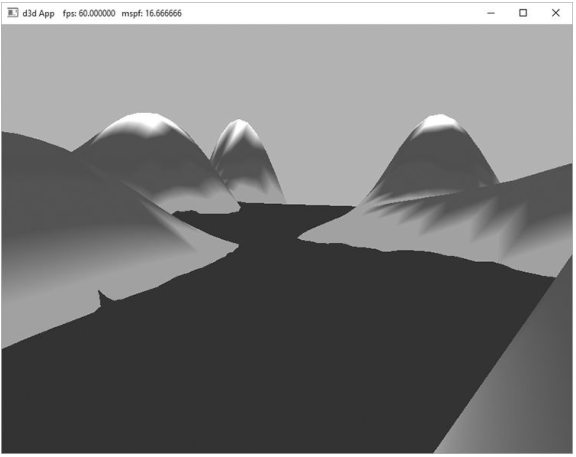
\includegraphics[width=\textwidth]{7-7}
    \centering
    \caption{“Lands and Waves”演示的屏幕截图。 因为我们还没有照明,所以很难看到波浪的形状。 按住“1”键可以在线框模式下查看场景,以更好地查看波形。}
    \label{fig:7-7}
\end{figure}

\begin{flushleft}
“漂亮”的实值(real-valued)函数$y=f(x,z)$的图是表面。 我们可以通过在$xz$平面中构建网格来近似表面,其中每个四边形由两个三角形构成,然后将函数应用于每个网格点; 见图\ref{fig:7-8}。
\end{flushleft}

\begin{figure}[h]
    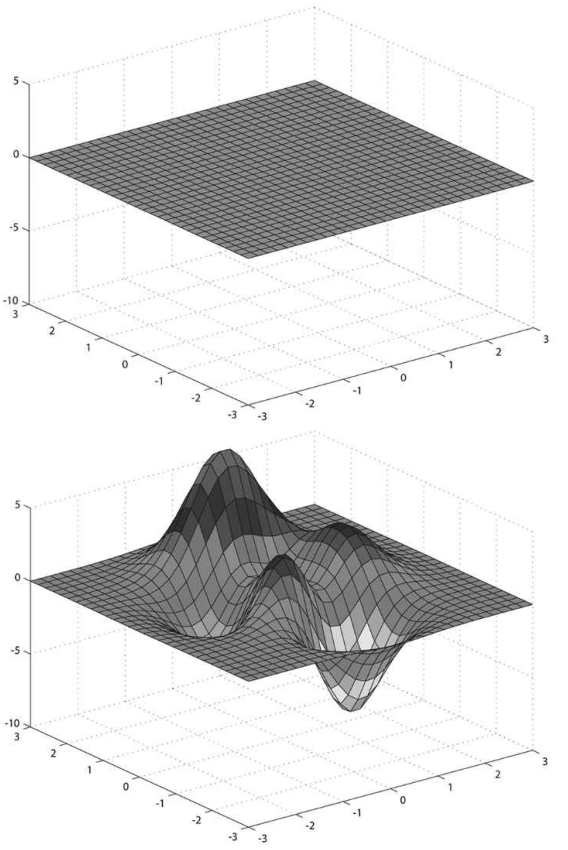
\includegraphics[width=\textwidth]{7-8}
    \centering
    \caption{(顶部)在xz平面中放置网格。(底部)对于每个网格点,应用函数f(x,z)以获得y坐标。 点(x,f(x,z),z)的图给出了曲面图。}
    \label{fig:7-8}
\end{figure}

%---- 7.7.1 ----
\subsection{创建网格顶点(Generating the Grid Vertices)}
\begin{flushleft}
因此,主要任务是如何在$xz$平面中构建网格。 $m\times n$顶点的网格,也就是$(m-1)\times(n-1)$个四边形(或单元),如图\ref{fig:7-9}所示。 每个单元格将被两个三角形覆盖,因此总共有2个$(m-1)\times(n-1)$个三角形。 如果网格具有宽度$w$和深度$d$,则沿$x$轴的单元间隔是$dx=w/(n-1)$,并且沿z轴的单元间隔是$dz=d/(m-1)$。 为了生成顶点,我们从左上角开始逐行逐行计算顶点坐标。 $xz$平面中第$i$个网格顶点的坐标由下式给出:\\
\end{flushleft}

\begin{align*}
v_{ij}=[-0.5w+j\cdot dx,0.0,0.5d-i\cdot dz]
\end{align*}

\begin{figure}[h]
    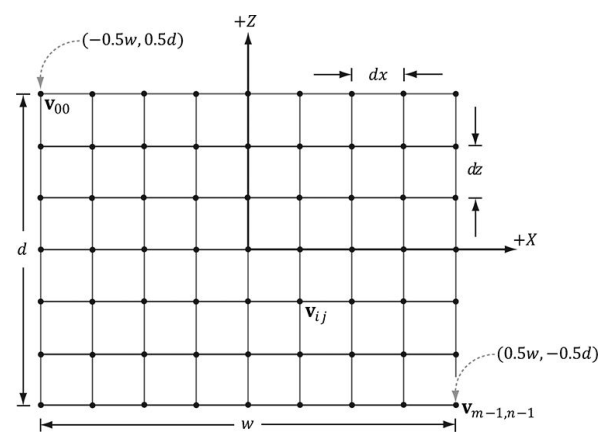
\includegraphics[width=\textwidth]{7-9}
    \centering
    \caption{网格构建}
    \label{fig:7-9}
\end{figure}

\begin{flushleft}
下面代码创建了这些个网格顶点:\\
\end{flushleft}

\begin{lstlisting}
GeometryGenerator::MeshData 
GeometryGenerator::CreateGrid(
    float width, 
    float depth, 
    uint32 m, 
    uint32 n)
{
    MeshData meshData;

    uint32 vertexCount = m*n;
    uint32 faceCount   = (m-1)*(n-1)*2;

    //
    // Create the vertices.
    //

    float halfWidth = 0.5f*width;
    float halfDepth = 0.5f*depth;

    float dx = width / (n-1);
    float dz = depth / (m-1);

    float du = 1.0f / (n-1);
    float dv = 1.0f / (m-1);

    meshData.Vertices.resize(vertexCount);
    for(uint32 i = 0; i < m; ++i)
    {
        float z = halfDepth - i*dz;
        for(uint32 j = 0; j < n; ++j)
        {
            float x = -halfWidth + j*dx;

            meshData.Vertices[i*n+j].Position = 
                XMFLOAT3(x, 0.0f, z);
            meshData.Vertices[i*n+j].Normal   = 
                XMFLOAT3(0.0f, 1.0f, 0.0f);
            meshData.Vertices[i*n+j].TangentU = 
                XMFLOAT3(1.0f, 0.0f, 0.0f);

            // Stretch texture over grid.
            meshData.Vertices[i*n+j].TexC.x = j*du;
            meshData.Vertices[i*n+j].TexC.y = i*dv;
        }
    }
......
\end{lstlisting}

%---- 7.7.2 ----
\subsection{创建网格索引(Generating the Grid Indices)}
\begin{flushleft}
在我们计算了顶点之后,我们需要通过指定索引来定义网格三角形。 为此,我们迭代每个四边形,从左上角开始逐行,并计算索引以定义四边形的两个三角形; 参考图\ref{fig:7-10},对于$m\times n$顶点网格,两个三角形的线性数组索引计算如下:\\
\end{flushleft}

\begin{align*}
\Delta ABC&=(i\cdot n+j,i\cdot n+j+1,(i+1)\cdot n+j)\\
\Delta CBD&=((i+1)\cdot n+j,i\cdot n+j+1,(i+1)\cdot n+j+1)
\end{align*}

\begin{figure}[h]
    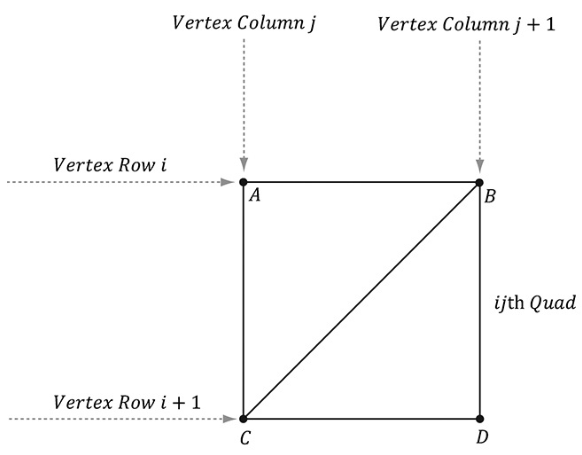
\includegraphics[width=\textwidth]{7-10}
    \centering
    \caption{网格构建}
    \label{fig:7-10}
\end{figure}

\begin{flushleft}
对应的代码如下:\\
\end{flushleft}

\begin{lstlisting}
//
// Create the indices.
//

meshData.Indices32.resize(faceCount*3); // 3 indices per face

// Iterate over each quad and compute indices.
uint32 k = 0;
for(uint32 i = 0; i < m-1; ++i)
{
    for(uint32 j = 0; j < n-1; ++j)
    {
        meshData.Indices32[k]   = i*n+j;
        meshData.Indices32[k+1] = i*n+j+1;
        meshData.Indices32[k+2] = (i+1)*n+j;

        meshData.Indices32[k+3] = (i+1)*n+j;
        meshData.Indices32[k+4] = i*n+j+1;
        meshData.Indices32[k+5] = (i+1)*n+j+1;

        k += 6; // next quad
    }
}
\end{lstlisting}

%---- 7.7.3 ----
\subsection{应用高度函数(Applying the Height Function)}
\begin{lstlisting}
// Not to be confused with GeometryGenerator::Vertex.
struct Vertex
{
    XMFLOAT3 Pos;
    XMFLOAT4 Color;
};
void LandAndWavesApp::BuildLandGeometry()
{
    GeometryGenerator geoGen;
    GeometryGenerator::MeshData grid = 
        geoGen.CreateGrid(160.0f, 160.0f, 50, 50);

    //
    // Extract the vertex elements we are 
    // interested and apply the height function to
    // each vertex.  In addition, color the vertices
    // based on their height so we have
    // sandy looking beaches, grassy low hills, 
    // and snow mountain peaks.
    //

    std::vector<Vertex> vertices(grid.Vertices.size());
    for(size_t i = 0; i < grid.Vertices.size(); ++i)
    {
        auto& p = grid.Vertices[i].Position;
        vertices[i].Pos = p;
        vertices[i].Pos.y = GetHillsHeight(p.x, p.z);

        // Color the vertex based on its height.
        if(vertices[i].Pos.y < -10.0f)
        {
            // Sandy beach color.
            vertices[i].Color = XMFLOAT4(1.0f, 0.96f, 0.62f, 1.0f);
        }
        else if(vertices[i].Pos.y < 5.0f)
        {
            // Light yellow-green.
            vertices[i].Color = XMFLOAT4(0.48f, 0.77f, 0.46f, 1.0f);
        }
        else if(vertices[i].Pos.y < 12.0f)
        {
            // Dark yellow-green.
            vertices[i].Color = XMFLOAT4(0.1f, 0.48f, 0.19f, 1.0f);
        }
        else if(vertices[i].Pos.y < 20.0f)
        {
            // Dark brown.
            vertices[i].Color = XMFLOAT4(0.45f, 0.39f, 0.34f, 1.0f);
        }
        else
        {
            // White snow.
            vertices[i].Color = XMFLOAT4(1.0f, 1.0f, 1.0f, 1.0f);
        }
    }
    
    const UINT vbByteSize = (UINT)vertices.size() * sizeof(Vertex);

    std::vector<std::uint16_t> indices = grid.GetIndices16();
    const UINT ibByteSize = (UINT)indices.size() * sizeof(std::uint16_t);

    auto geo = std::make_unique<MeshGeometry>();
    geo->Name = "landGeo";

    ThrowIfFailed(D3DCreateBlob(vbByteSize, &geo->VertexBufferCPU));
    CopyMemory(geo->VertexBufferCPU->GetBufferPointer(), 
        vertices.data(), vbByteSize);

    ThrowIfFailed(D3DCreateBlob(ibByteSize, &geo->IndexBufferCPU));
    CopyMemory(geo->IndexBufferCPU->GetBufferPointer(), 
        indices.data(), ibByteSize);

    geo->VertexBufferGPU = d3dUtil::CreateDefaultBuffer(md3dDevice.Get(),
        mCommandList.Get(), vertices.data(), vbByteSize, 
        geo->VertexBufferUploader);

    geo->IndexBufferGPU = d3dUtil::CreateDefaultBuffer(md3dDevice.Get(),
        mCommandList.Get(), indices.data(), ibByteSize, 
        geo->IndexBufferUploader);

    geo->VertexByteStride = sizeof(Vertex);
    geo->VertexBufferByteSize = vbByteSize;
    geo->IndexFormat = DXGI_FORMAT_R16_UINT;
    geo->IndexBufferByteSize = ibByteSize;

    SubmeshGeometry submesh;
    submesh.IndexCount = (UINT)indices.size();
    submesh.StartIndexLocation = 0;
    submesh.BaseVertexLocation = 0;

    geo->DrawArgs["grid"] = submesh;

    mGeometries["landGeo"] = std::move(geo);
}
\end{lstlisting}

\begin{flushleft}
(GetHillsHeight)函数 f(x,z) 如下:\\
\end{flushleft}

\begin{lstlisting}
float LandAndWavesApp::GetHillsHeight(float x, float z)const
{
    return 0.3f*(z*sinf(0.1f*x) + x*cosf(0.1f*z));
}
\end{lstlisting}

\begin{flushleft}
它的图形看起来有点像山丘和山谷的地形(见图\ref{fig:7-7})。
\end{flushleft}

%---- 7.7.4 ----
\subsection{根常量缓冲区视图(Root CBVs)}
\begin{flushleft}
我们在“Land and Waves”演示所做的另一项更改(对比“Shape”演示)是我们使用根描述符,以便我们可以直接绑定CBV而无需使用描述符堆。 以下是需要进行的更改:\\
\end{flushleft}

\begin{itemize}
  \item 1.需要更改根签名以获取两个根CBV而不是两个描述符表。
  \item 2.不需要CBV堆也不需要使用描述符填充。
  \item 3.绑定根描述符有新的语法。
\end{itemize}

\begin{flushleft}
新的根签名是这样定义的:\\
\end{flushleft}

\begin{lstlisting}
// Root parameter can be a table, root descriptor or root constants.
CD3DX12_ROOT_PARAMETER slotRootParameter[2];

// Create root CBV.
slotRootParameter[0].InitAsConstantBufferView(0);
slotRootParameter[1].InitAsConstantBufferView(1);

// A root signature is an array of root parameters.
CD3DX12_ROOT_SIGNATURE_DESC rootSigDesc(2, slotRootParameter, 
    0, nullptr, 
    D3D12_ROOT_SIGNATURE_FLAG_ALLOW_INPUT_ASSEMBLER_INPUT_LAYOUT);
\end{lstlisting}

\begin{flushleft}
注意我们使用 InitAsConstantBufferView 辅助方法来创建根CBV; 该参数指定此参数绑定的着色器寄存器(在上面的代码中,着色器常量缓冲寄存器“b0”和“b1”)。\\
现在,我们使用以下方法将CBV作为参数绑定到根描述符:\\
\end{flushleft}

\begin{lstlisting}
void ID3D12GraphicsCommandList::
    SetGraphicsRootConstantBufferView(
        UINT RootParameterIndex,
        D3D12_GPU_VIRTUAL_ADDRESS BufferLocation);
\end{lstlisting}

\begin{itemize}
  \item 1.RootParameterIndex: 绑定CBV的根参数的索引。
  \item 2.BufferLocation: 包含常量缓冲区数据的资源的虚拟地址。
\end{itemize}

\begin{flushleft}
基于这些变化,绘制的代码现在变成这样:\\
\end{flushleft}

\begin{lstlisting}
void LandAndWavesApp::Draw(const GameTimer& gt)
{
    ......

    // Bind per-pass constant buffer.  We only need to do this once per-pass.
    auto passCB = mCurrFrameResource->PassCB->Resource();
    mCommandList->SetGraphicsRootConstantBufferView(1, 
        passCB->GetGPUVirtualAddress());

    DrawRenderItems(mCommandList.Get(), 
        mRitemLayer[(int)RenderLayer::Opaque]);

    ......
}

void LandAndWavesApp::DrawRenderItems(
    ID3D12GraphicsCommandList* cmdList, 
    const std::vector<RenderItem*>& ritems)
{
    UINT objCBByteSize = d3dUtil::CalcConstantBufferByteSize(
        sizeof(ObjectConstants));

    auto objectCB = mCurrFrameResource->ObjectCB->Resource();

    // For each render item...
    for(size_t i = 0; i < ritems.size(); ++i)
    {
        auto ri = ritems[i];

        cmdList->IASetVertexBuffers(0, 1, 
            &ri->Geo->VertexBufferView());
        cmdList->IASetIndexBuffer(
            &ri->Geo->IndexBufferView());
        cmdList->IASetPrimitiveTopology(
            ri->PrimitiveType);

        D3D12_GPU_VIRTUAL_ADDRESS objCBAddress = 
            objectCB->GetGPUVirtualAddress();
        objCBAddress += ri->ObjCBIndex*objCBByteSize;

        cmdList->SetGraphicsRootConstantBufferView(0, 
            objCBAddress);

        cmdList->DrawIndexedInstanced(ri->IndexCount, 
            1, ri->StartIndexLocation, 
            ri->BaseVertexLocation, 0);
    }
}
\end{lstlisting}


%---- 7.7.5 ----
\subsection{动态顶点缓冲区(Dynamic Vertex Buffers)}
\begin{flushleft}
到目前为止,我们已将顶点存储在默认缓冲区资源中。当我们想要存储静态几何时,我们使用这种资源。也就是说,我们不改变的几何 - 设置数据,GPU读取和绘制数据。动态顶点缓冲区是我们频繁更改顶点数据的地方,比如每帧。例如,假设我们正在进行波浪模拟,我们求解解函数$f(x,z,t)$的波动方程。该函数表示在时间$t$的$xz$平面中每个点处的波高。如果我们使用这个函数来绘制波浪,我们将像使用峰和谷一样使用三角形网格网格,并将$f(x,z,t)$应用于每个网格点,以获得波高。网格点。因为此函数还取决于时间$t$(即,波面随时间变化),我们需要在短时间后(例如每1/30秒)将此函数重新应用于网格点以获得平滑动画。因此,我们需要一个动态顶点缓冲区,以便随着时间的推移更新三角形网格网格顶点的高度。导致动态顶点缓冲的另一种情况是具有复杂物理和碰撞检测的粒子系统。我们将在每个帧上对CPU进行物理和碰撞检测,以找到粒子的新位置。因为粒子位置正在改变每一帧,我们需要一个动态顶点缓冲区来更新粒子位置以绘制每一帧。\\

我们已经看到了一个示例,当我们使用上传缓冲区来更新我们的常量缓冲区数据时,将数据从CPU上传到GPU。 我们可以应用相同的技术并使用我们的UploadBuffer类,但不是存储常量缓冲区数组,而是存储顶点数组:\\
\end{flushleft}

\begin{lstlisting}
std::unique_ptr<UploadBuffer<Vertex>> WavesVB = nullptr;
WavesVB = std::make_unique<UploadBuffer<Vertex>>(
    device, waveVertCount, false);
\end{lstlisting}

\begin{flushleft}
因为我们需要每帧将新内容从 CPU 上传到 wave 的动态顶点缓冲区,所以动态顶点缓冲区需要是帧资源。 否则,我们可以在 GPU 处理完最后一帧之前覆盖内存。\\
每一帧,我们运行波浪模拟并更新顶点缓冲区,如下所示:\\
\end{flushleft}

\begin{lstlisting}
void LandAndWavesApp::UpdateWaves(const GameTimer& gt)
{
	// Every quarter second, generate a random wave.
	static float t_base = 0.0f;
	if((mTimer.TotalTime() - t_base) >= 0.25f)
	{
		t_base += 0.25f;

		int i = MathHelper::Rand(4, 
            mWaves->RowCount() - 5);
		int j = MathHelper::Rand(4,
            mWaves->ColumnCount() - 5);

		float r = MathHelper::RandF(0.2f, 0.5f);

		mWaves->Disturb(i, j, r);
	}

	// Update the wave simulation.
	mWaves->Update(gt.DeltaTime());

	// Update the wave vertex buffer with the new solution.
	auto currWavesVB = mCurrFrameResource->WavesVB.get();
	for(int i = 0; i < mWaves->VertexCount(); ++i)
	{
		Vertex v;

		v.Pos = mWaves->Position(i);
        v.Color = XMFLOAT4(DirectX::Colors::Blue);

		currWavesVB->CopyData(i, v);
	}

	// Set the dynamic VB of the wave renderitem to the current frame VB.
	mWavesRitem->Geo->VertexBufferGPU = currWavesVB->Resource();
}
\end{lstlisting}

\begin{flushleft}
NOTICE: 我们保存对波渲染项(mWavesRitem)的引用,以便我们可以动态设置其顶点缓冲区。 我们需要这样做,因为它的顶点缓冲区是一个动态缓冲区并且每帧都会改变。\\

使用动态缓冲区时会有一些开销,因为必须将新数据从CPU内存传输回GPU内存。 因此,静态缓冲区应该优先于动态缓冲区,前提是静态缓冲区可以工作。 最新版本的Direct3D引入了新功能,以减少对动态缓冲区的需求。 例如:\\
\end{flushleft}

\begin{itemize}
  \item 1.可以在顶点着色器中完成简单动画。
  \item 2.通过渲染到纹理或计算着色器和顶点纹理获取功能,可以实现像上面描述的完全在GPU上运行的波模拟。
  \item 3.几何着色器为GPU提供了创建或销毁基元的能力,这是一项通常需要在没有几何着色器的情况下在CPU上完成的任务。
  \item 4.曲面细分阶段可以在GPU上添加细分几何体,这通常需要在没有硬件细分的情况下在CPU上完成。
\end{itemize}

\begin{flushleft}
索引缓冲区也可以是动态的。 然而,在“Land and Waves”演示中,三角形拓扑保持不变,只有顶点高度发生变化; 因此,只有顶点缓冲区需要是动态的。\\
本章的“Waves”演示使用动态顶点缓冲区来实现一个简单的波浪模拟,就像本节开头所描述的那样。 对于本书,我们不关心波模拟的实际算法细节(参见[Lengyel02]),但更多的是使用该过程来说明动态缓冲区:更新CPU上的模拟,然后使用更新顶点数据 上传缓冲区。\\
~\\
NOTICE: 我们再次提到,这个演示可以使用更高级的方法在GPU上实现,例如渲染到纹理功能或计算着色器,以及顶点纹理提取。 因为我们尚未涉及这些主题,所以我们在CPU上进行波浪模拟,并使用动态顶点缓冲区更新新顶点。
\end{flushleft}



%---- 7.8 ----
\section{总结}
\begin{flushleft}
1.等待GPU每帧执行队列中的所有命令都是低效的,因为它会导致CPU和GPU在某个时刻空闲。 更有效的技术是创建帧资源 - CPU需要修改每个帧的资源的循环数组。 这样,CPU在进入下一帧之前不需要等待GPU完成; CPU将仅与下一个可用(即,未被GPU使用)帧资源一起工作。 如果CPU总是以比GPU更快的速度处理帧,那么最终CPU将不得不在某个时刻等待GPU赶上,但这是理想的情况,因为GPU正在被充分利用; 额外的CPU周期总是可以用于游戏的其他部分,如AI,物理和游戏逻辑。\\
2.我们可以使用 ID3D12DescriptorHeap::GetCPUDescriptorHandleForHeapStart 方法获取堆中第一个描述符的句柄。我们可以使用 ID3D12Device::GetDescriptorHandleIncrementSize (DescriptorHeapType类型)方法获取描述符大小(取决于硬件和描述符类型)。 一旦我们知道描述符增量大小,我们就可以使用两个 CD3DX12\_CPU\_DESCRIPTOR\_HANDLE::Offset 方法之一来通过 n 个描述符来偏移句柄:\\
\end{flushleft}

\begin{lstlisting}
// Specify the number of descriptors to 
// offset times the descriptor
// increment size:
D3D12_CPU_DESCRIPTOR_HANDLE handle = mCbvHeap->
    GetCPUDescriptorHandleForHeapStart();
handle.Offset(n * mCbvSrvDescriptorSize);
// Or equivalently, specify the number of 
// descriptors to offset,
// followed by the descriptor increment size:
D3D12_CPU_DESCRIPTOR_HANDLE handle = mCbvHeap->
    GetCPUDescriptorHandleForHeapStart();
handle.Offset(n, mCbvSrvDescriptorSize);
// The CD3DX12_GPU_DESCRIPTOR_HANDLE type has 
// the same Offset methods.
\end{lstlisting}

\begin{flushleft}
3.根签名定义了在发出绘制调用之前需要将哪些资源绑定到管道以及这些资源如何映射到着色器输入寄存器。需要绑定哪些资源取决于绑定着色器程序所期望的资源。创建PSO时,将验证根签名和着色器程序组合。根签名被指定为根参数数组。根参数可以是描述符表,根描述符或根常量。描述符表指定堆中的连续描述符范围。根描述符用于直接在根签名中绑定描述符(它不需要在堆中)。根常量用于直接在根签名中绑定常量值。为了提高性能,可以将64个DWORD限制在根签名中。描述符表每个花费一个DWORD,根描述符每个花费两个DWORD,根常量为每个32位常量花费一个DWORD。硬件会自动保存每个绘制调用的根参数的快照。因此,我们可以安全地更改每个绘制调用的根参数,但是,我们还应该尝试保持根签名较小,以便复制更少的内存。\\
4.当需要在运行时频繁更新顶点缓冲区的内容时(例如,每帧或每1/30秒),使用动态顶点缓冲区。 我们可以使用UploadBuffer来实现动态顶点缓冲区,但是我们存储了一个顶点数组,而不是存储常量缓冲区数组。 因为我们需要每帧将新内容从 CPU 上传到 wave 的动态顶点缓冲区,所以动态顶点缓冲区需要是帧资源。 使用动态顶点缓冲区时会有一些开销,因为新数据必须从CPU内存传输回GPU内存。 因此,静态顶点缓冲区应该优先于动态顶点缓冲区,前提是静态顶点缓冲区可以工作。 最新版本的Direct3D引入了新功能,以减少对动态缓冲区的需求。\\
\end{flushleft}

%---- 7.9 ----
\section{练习}
\begin{flushleft}
1.修改“Shapes”演示以使用 GeometryGenerator::CreateGeosphere 而不是 GeometryGenerator::CreateSphere。 尝试使用0,1,2和3细分级别。\\
2.修改“Shapes”演示以使用十六个根常量来设置每个对象的世界矩阵而不是描述符表。\\
3.在DVD上,有一个名为 Models/Skull.txt 的文件。 该文件包含图\ref{fig:7-11}中渲染头骨所需的顶点和索引列表。 使用文本编辑器(如记事本)研究文件,并修改“形状”演示以加载和渲染头骨网格。
\end{flushleft}

\begin{figure}[h]
    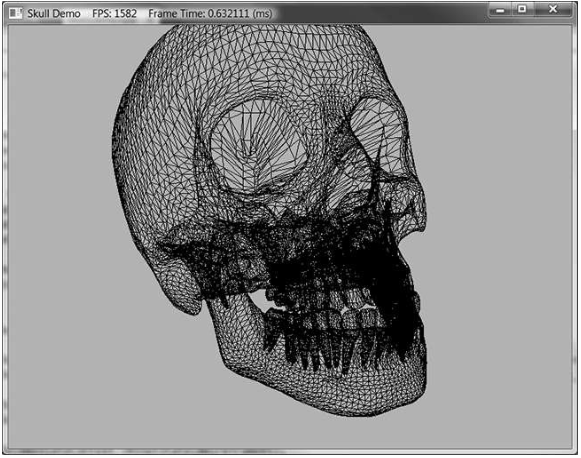
\includegraphics[width=\textwidth]{7-11}
    \centering
    \caption{练习3的渲染输出}
    \label{fig:7-11}
\end{figure}













